\documentclass{beamer} % only slides
%\documentclass[notes]{beamer} % slides + notes
\geometry{paperwidth=140mm,paperheight=105mm}

\usepackage[utf8]{inputenc}
\usepackage[%
  backend=biber,
  url=false,
  style=authoryear,
  citestyle=authoryear,
  uniquelist=false,
  maxnames=2,
  minnames=1,
  maxbibnames=99,
  giveninits,
  dashed=false]{biblatex} % TODO: adapt citation style
\renewcommand*{\nameyeardelim}{\addcomma\space}

\usepackage{amsfonts}
\usepackage{amsmath,amssymb}
\usepackage{amsthm}

\usepackage[normalem]{ulem}

\usepackage{mathtools}
\DeclarePairedDelimiter\abs{\lvert}{\rvert}%
\usepackage{enumerate}
% \usepackage{caption}
% \usepackage{subcaption}
% \usepackage{xcolor}
% \usepackage{graphicx}
% \graphicspath{ {./imgs/} }
\usepackage{tikz}
\usetikzlibrary{scopes,calc,shapes.misc,bending,positioning,intersections,through,backgrounds}

\tikzset{
  graphNode/.style={circle,fill,inner sep=0.05cm},
  edgeLabel/.style={circle,inner sep=0.05cm,fill=white},
  mstEdge/.style={draw=mygreen,very thick},
  mstEdgeLabel/.style={edgeLabel,text=mygreen},
  addedEdge/.style={draw=mybluegreen,very thick},
  addedEdgeLabel/.style={edgeLabel,text=mybluegreen},
  inactiveEdge/.style={draw=mygrey},
  inactiveEdgeLabel/.style={edgeLabel,text=mygrey},
  currentNode/.style={circle,draw=myred,very thick},
  currentEdge/.style={draw=myblue,very thick},
  resultEdge/.style={draw=myblue,very thick},
  resultEdgeLabel/.style={edgeLabel,text=myblue},
  connect/.style={rounded corners=#1,
      to path= ($(\tikztostart)!-#1!(\tikztotarget)!-#1!-90:(\tikztotarget)$) -- ($(\tikztotarget)!-#1!(\tikztostart)!-#1!90:(\tikztostart)$) --
      ($(\tikztotarget)!-#1!(\tikztostart)!#1!90:(\tikztostart)$) -- ($(\tikztostart)!-#1!(\tikztotarget)!-#1!90:(\tikztotarget)$) -- cycle (\tikztotarget)
    },
  pics/He/.style n args={4}{code={
    \node at (-0.25,0.5*\HeHeight) {{#1}};
    \node at (0.25+\HeWidth,0.5*\HeHeight) {{#2}};
    \node[graphNode,#3] at (0,\HeHeight) (-u1) {};
    \node[graphNode] at (0.5*\HeWidth,\HeHeight) (-u3) {};
    \node[graphNode,#4] at (\HeWidth,\HeHeight) (-v2) {};
    \node[graphNode] at (0,0.66*\HeHeight) (-u4) {};
    \node[graphNode] at (0.5*\HeWidth,0.66*\HeHeight) (-v6) {};
    \node[graphNode] at (\HeWidth,0.66*\HeHeight) (-u5) {};
    \node[graphNode] at (0,0.33*\HeHeight) (-v5) {};
    \node[graphNode] at (0.5*\HeWidth,0.33*\HeHeight) (-u6) {};
    \node[graphNode] at (\HeWidth,0.33*\HeHeight) (-v4) {};
    \node[graphNode,#3] at (0,0) (-u2) {};
    \node[graphNode] at (0.5*\HeWidth,0) (-v3) {};
    \node[graphNode,#4] at (\HeWidth,0) (-v1) {};
  
    \path[-] (-u1) edge (-u3);
    \path[-] (-u1) edge (-u4);
    \path[-] (-u2) edge (-v3);
    \path[-] (-u2) edge (-v5);
    \path[-] (-u3) edge (-v2);
    \path[-] (-u4) edge (-v5);
    \path[-] (-u4) edge (-v6);
    \path[-] (-u5) edge (-v2);
    \path[-] (-u5) edge (-v4);
    \path[-] (-u5) edge (-v6);
    \path[-] (-u6) edge (-v4);
    \path[-] (-u6) edge (-v5);
    \path[-] (-v1) edge (-v3);
    \path[-] (-v1) edge (-v4);}},
  lrRandomEdge/.style={draw=myorange,very thick},
  lrRandomEdge on/.style={alt={#1{lrRandomEdge}{}}},
  lr1Edge/.style={draw=mygreen,very thick},
  lr1Edge on/.style={alt={#1{lr1Edge}{}}},
  lr1EdgeLabel/.style={edgeLabel,text=mygreen},
  lr4Edge/.style={draw=myblue,very thick},
  lr4Edge on/.style={alt={#1{lr4Edge}{}}},
  lr4EdgeLabel/.style={label={[label distance=-0.15cm]below:{\footnotesize\color{myblue} 4}}},
  lr5Edge/.style={draw=mypurple,very thick},
  lr5Edge on/.style={alt={#1{lr5Edge}{}}},
  lr5EdgeLabel/.style={edgeLabel,text=mypurple},
  hpStartNode on/.style={alt={#1{fill=mygreen}{}}},
  inactiveEdges on/.style={alt={#1{every edge/.append style={inactiveEdge}}{}}},
  invisible/.style={opacity=0},
  visible on/.style={alt={#1{}{invisible}}},
  invisible on/.style={alt={#1{invisible}{}}},
  text invisible/.style={text opacity=0},
  text visible on/.style={alt={#1{}{text invisible}}},
  alt/.code args={<#1>#2#3}{%
    \alt<#1>{\pgfkeysalso{#2}}{\pgfkeysalso{#3}} % \pgfkeysalso doesn't change the path
  },
}

\usepackage{float}
\usepackage{verbatim}
\usepackage{datetime}
\usepackage{transparent}

\usepackage{array}
\usepackage{makecell}
\renewcommand{\theadalign}{tr}
\renewcommand\theadfont{\itshape}
\renewcommand{\cellalign}{tl}

% \theoremstyle{definition}
% \newtheorem{definition}{Definition}
% \newtheorem{theorem}{Theorem}

% appendix numbering
\newcommand{\backupbegin}{
   \newcounter{framenumberappendix}
   \setcounter{framenumberappendix}{\value{framenumber}}
}
\newcommand{\backupend}{
   \addtocounter{framenumberappendix}{-\value{framenumber}}
   \addtocounter{framenumber}{\value{framenumberappendix}} 
}

\newenvironment{proofIdea}{%
  \renewcommand{\proofname}{Proof Idea}\renewcommand{\qedsymbol}{}\proof}{\endproof}

\newcommand\blfootnote[1]{%
  \begingroup
  \renewcommand\thefootnote{}\footnote{#1}%
  \addtocounter{footnote}{-1}%
  \endgroup
}

% \newcommand{\P}{\textsc{P}}
\newcommand{\NP}{\textsc{NP}}
\newcommand{\maxSNP}{\textsc{MaxSNP}}

\newcommand{\TSP}{\textsc{TSP}}
\newcommand{\mTSP}{\textsc{Metric TSP}}
\newcommand{\VC}{\textsc{VC}}

% tikz stuff colors
\colorlet{myred}{red!80!yellow}
\colorlet{myblue}{blue!75!white!75!green}
\colorlet{mygreen}{green!80!blue}
\colorlet{mybluegreen}{blue!50!green!70!white}
\colorlet{myyellow}{yellow!70!red}
\colorlet{myorange}{red!70!yellow}
\colorlet{mypurple}{red!50!blue!70!white}
\colorlet{mygrey}{black!30!white}

\newcommand{\HeWidth}{1.5}
\newcommand{\HeHeight}{1}
\newcommand{\HeMargin}{0.5}

\beamertemplatenavigationsymbolsempty
\setbeamertemplate{footline}{Formalizing Theory of Approximating the Traveling-Salesman Problem, Lukas Koller\hfill \insertframenumber{}/\inserttotalframenumber}
\setbeamercovered{transparent}

\title{Formalizing Theory of Approximating the Traveling-Salesman Problem}
\subtitle{Interdisciplinary Project, Mathematics}
\author{Lukas Koller}
\date{\today}

\bibliography{refs}

\begin{document}

\frame{\titlepage}

% \begin{frame}
%   \frametitle{Traveling-Salesman Problem}

%   \begin{figure}
%     \centering
%     \def\svgwidth{0.9\textwidth}{\tiny\input{imgs/munich_ubahn.pdf_tex}}%
%     \caption{Munich U-Bahn network.}
%   \end{figure}

%   \note[item]{ A friend visits you in Munich for an afternoon. You want to show her/him some sights in Munich, e.g. your university in Garching, Marienplatz, Olympia Park, etc..}
%   \note[item]{ Unfortunately, your friend has to catch a train at Hauptbahnhof in the }
% \end{frame}

\begin{frame}
  \frametitle{Traveling-Salesman Problem}

  The \textsc{Traveling-Salesman Problem} (\TSP{}) is a well known combinatorial optimization problem.

  \onslide<2->{
    \begin{columns}[T] % align columns
      \begin{column}{.25\textwidth}
        \begingroup
        \tikzset{every picture/.style={scale=0.7}}%
        \begin{figure}
          \begin{overprint}
            \onslide<1-2>\begin{center}\newcommand*{\circleDia}{2.0cm}
\newcommand*{\edgeBend}{0}
\newcommand*{\etMargin}{0.15cm}

\begin{tikzpicture}[label distance=0mm,scale=1]
  \foreach \a in {1,2,...,5}{
      \draw (90+144-\a*360/5: \circleDia) node[graphNode,label={90+144-\a*360/5:$\mathstrut \a$}] (\a) {};
    }

  \path[-] (1) edge node[edgeLabel] {\footnotesize $2$} (2);
  \path[-] (1) edge node[edgeLabel] {\footnotesize $3$} (3);
  \path[-] (1) edge node[edgeLabel] {\footnotesize $3$} (4);
  \path[-] (1) edge node[edgeLabel] {\footnotesize $3$} (5);

  \path[-] (2) edge node[edgeLabel] {\footnotesize $2$} (3);
  \path[-] (2) edge node[edgeLabel] {\footnotesize $3$} (4);
  \path[-] (2) edge node[edgeLabel] {\footnotesize $1$} (5);

  \path[-] (3) edge node[edgeLabel] {\footnotesize $3$} (4);
  \path[-] (3) edge node[edgeLabel] {\footnotesize $2$} (5);

  \path[-] (4) edge node[edgeLabel] {\footnotesize $2$} (5);

\end{tikzpicture}
\end{center}
            \onslide<3->\begin{center}\newcommand*{\circleDia}{2.0cm}
\newcommand*{\edgeBend}{15}

\begin{tikzpicture}[label distance=0mm,scale=1]
  \foreach \a in {1,2,...,5}{
      \draw (90+144-\a*360/5: \circleDia) node[graphNode,label={90+144-\a*360/5:$\mathstrut \a$}] (\a) {};
    }

  % \path[-] (1) edge node[edgeLabel] {\footnotesize $2$} (2);
  \path[-] (1) edge[resultEdge] node[resultEdgeLabel] {\footnotesize $2$} (2);
  \path[-] (1) edge[inactiveEdge] node[inactiveEdgeLabel] {\footnotesize $3$} (3);
  % \path[-] (1) edge[resultEdge] node[resultEdgeLabel] {\footnotesize $3$} (4);
  \path[-] (1) edge[inactiveEdge] node[inactiveEdgeLabel] {\footnotesize $3$} (5);

  % \path[-] (2) edge node[edgeLabel] {\footnotesize $2$} (3);
  \path[-] (2) edge[resultEdge] node[resultEdgeLabel] {\footnotesize $2$} (3);
  \path[-] (2) edge[inactiveEdge] node[inactiveEdgeLabel] {\footnotesize $3$} (4);
  % \path[-] (2) edge node[edgeLabel] {\footnotesize $1$} (5);
  \path[-] (2) edge[inactiveEdge] node[inactiveEdgeLabel] {\footnotesize $1$} (5);

  \path[-] (3) edge[inactiveEdge] node[inactiveEdgeLabel] {\footnotesize $3$} (4);
  \path[-] (3) edge[resultEdge] node[resultEdgeLabel] {\footnotesize $2$} (5);

  % \path[-] (4) edge node[edgeLabel] {\footnotesize $2$} (5);
  \path[-] (4) edge[resultEdge] node[resultEdgeLabel] {\footnotesize $2$} (5);

  \path[-] (1) edge[resultEdge] node[resultEdgeLabel] {\footnotesize $3$} (4);

\end{tikzpicture}
\end{center}
          \end{overprint}
        \end{figure}
        \endgroup
      \end{column}%
      \hfill%
      \begin{column}{.75\textwidth}
        \begin{minipage}[c][.4\textheight][c]{\linewidth}
          \begin{definition}[\textsc{Traveling-Salesman Problem}]
            \begin{tabular}{ r l }
              \thead{Input:} & \makecell{undirected graph $G$ with            \\ edge weights $c:E(G)\to\mathbb{R}_+$.} \\
              \thead{Task:}  & \makecell{Find a Hamiltonian cycle in $G$ with \\ minimum total weight.}
            \end{tabular}
          \end{definition}
        \end{minipage}
      \end{column}%
    \end{columns}
  }
  \onslide<4->{
    \begin{theorem}[15.43, \cite{korte_vygen_2018}]
      The decision problem of \TSP{} is \NP{}-hard.
    \end{theorem}
  }
  \vspace*{0.5cm}
  \onslide<5->{
    {\color{myred} $\implies$ We can't solve \TSP{} optimally in polynomial time, unless $\textsc{P}=\NP{}$.}
  }
\end{frame}

\begin{frame}
  \frametitle{Approximation Algorithms for TSP}

  \begin{itemize}
    \item An \textit{approximation algorithm} is a polynomial-time algorithm for an optimization problem that returns an approximate solution.
    \item The \textit{approximation ratio} bounds the distance between the approximate solution and the optimal solution.
  \end{itemize}
  \vspace*{0.5cm}
  \pause
  {\color{myred} Negative result for \TSP{}:}
  \begin{theorem}[\cite{sahni_gonzalez_1976}]
    There is no constant-factor approx. algorithm for \TSP{}, unless $\textsc{P}=\NP{}$.
  \end{theorem}
  \vspace*{0.5cm}
  \pause
  We simplify the \TSP{} to the \mTSP{} by assuming:
  \begin{enumerate}[(i)]
    \item the graph $G$ is complete and
    \item the edge weights $c$ satisfy the triangle-inequality.
  \end{enumerate}
  \vspace*{0.5cm}
  \pause
  \begin{theorem}[\cite{sahni_gonzalez_1976}]
    The decision problem of \mTSP{} is \NP{}-hard.
  \end{theorem}

\end{frame}

\begin{frame}
  \frametitle{Overview}

  \begin{enumerate}[(i)]
    \item I have formalized a proof for the equivalence of the \textsc{Maximum Matching Problem} and the \textsc{Minimum Matching-Perfect Problem}.
  \end{enumerate}
  \vspace*{0.25cm}

  \pause
  I have formalized parts of the section 21.1, \textit{Approximation Algorithms for the TSP} from \parencite{korte_vygen_2018}.
  \vspace*{0.25cm}
  \begin{enumerate}[(i)]
    \setcounter{enumi}{1}
    \item<1,2-> I have formally verified two approx. algorithms for \mTSP{}.
      \begin{itemize}
        \item \textsc{DoubleTree} and \textsc{Christofides-Serdyukov} algorithm
      \end{itemize}
      \vspace*{0.25cm}
    \item<1,3-> I have formalized a L-reduction from \textsc{VCP4}\footnotemark{} to \mTSP{}.
      \begin{itemize}
        \item \textsc{VCP4} is \maxSNP{}-hard \parencite[Thm. 16.46,][]{korte_vygen_2018}\\ $\implies$ \mTSP{} is \maxSNP{}-hard.
      \end{itemize}
  \end{enumerate}
  \footnotetext[1]{\textsc{Minimum Vertex Cover Problem} with maximum degree of 4}
\end{frame}

\begin{frame}
  \frametitle{Christofides-Serdyukov Algorithm \parencite{christofides_1976,serdyukov_1978}}

  \begin{theorem}[21.5, \cite{korte_vygen_2018}]
    \textsc{Christofides-Serdyukov} is a $\frac{3}{2}$-approx. algorithm for \mTSP{}.
  \end{theorem}
  % \begin{proofIdea}
  %   The total weight of the minimum perfect-matching is at most half of the total weight of the optimal Hamiltonian cycle.
  % \end{proofIdea}

  \begin{columns}[T] % align columns
    \begin{column}{.35\textwidth}
      \begin{figure}
        \begin{overprint}
          \onslide<1>\begin{center}\newcommand*{\circleDia}{2.0cm}
\newcommand*{\edgeBend}{0}

\begin{tikzpicture}[label distance=0mm,scale=1]
  \foreach \a in {1,2,...,5}{
      \draw (90+144-\a*360/5: \circleDia) node[graphNode,label={90+144-\a*360/5:$\mathstrut \a$}] (\a) {};
    }

  \path[-] (1) edge node[edgeLabel] {\footnotesize $2$} (2);
  % \path[-] (1) edge[mstEdge] node[mstEdgeLabel] {\footnotesize $2$} (2);
  \path[-] (1) edge node[edgeLabel] {\footnotesize $3$} (3);
  \path[-] (1) edge node[edgeLabel] {\footnotesize $3$} (4);
  \path[-] (1) edge node[edgeLabel] {\footnotesize $3$} (5);

  \path[-] (2) edge node[edgeLabel] {\footnotesize $2$} (3);
  % \path[-] (2) edge[mstEdge,bend right=\edgeBend] node[mstEdgeLabel] {\footnotesize $2$} (3);
  % \path[-] (2) edge[mstEdge,bend left=\edgeBend] node[mstEdgeLabel] {\footnotesize $2$} (3);
  \path[-] (2) edge node[edgeLabel] {\footnotesize $3$} (4);
  \path[-] (2) edge node[edgeLabel] {\footnotesize $1$} (5);
  % \path[-] (2) edge[mstEdge] node[mstEdgeLabel] {\footnotesize $1$} (5);

  \path[-] (3) edge node[edgeLabel] {\footnotesize $3$} (4);
  \path[-] (3) edge node[edgeLabel] {\footnotesize $2$} (5);

  \path[-] (4) edge node[edgeLabel] {\footnotesize $2$} (5);
  % \path[-] (4) edge[mstEdge] node[mstEdgeLabel] {\footnotesize $2$} (5);

\end{tikzpicture}
\end{center}
          \onslide<2>\begin{center}\newcommand*{\circleDia}{2.0cm}
\newcommand*{\edgeBend}{0}

\begin{tikzpicture}[label distance=0mm,scale=1]
  \foreach \a in {1,2,...,5}{
      \draw (90+144-\a*360/5: \circleDia) node[graphNode,label={90+144-\a*360/5:$\mathstrut \a$}] (\a) {};
    }

  % \path[-] (1) edge node[edgeLabel] {\footnotesize $2$} (2);
  \path[-] (1) edge[mstEdge] node[mstEdgeLabel] {\footnotesize $2$} (2);
  \path[-] (1) edge[inactiveEdge] node[inactiveEdgeLabel] {\footnotesize $3$} (3);
  \path[-] (1) edge[inactiveEdge] node[inactiveEdgeLabel] {\footnotesize $3$} (4);
  \path[-] (1) edge[inactiveEdge] node[inactiveEdgeLabel] {\footnotesize $3$} (5);

  % \path[-] (2) edge node[edgeLabel] {\footnotesize $2$} (3);
  \path[-] (2) edge[mstEdge,bend right=\edgeBend] node[mstEdgeLabel] {\footnotesize $2$} (3);
  % \path[-] (2) edge[mstEdge,bend left=\edgeBend] node[mstEdgeLabel] {\footnotesize $2$} (3);
  \path[-] (2) edge[inactiveEdge] node[inactiveEdgeLabel] {\footnotesize $3$} (4);
  % \path[-] (2) edge node[edgeLabel] {\footnotesize $1$} (5);
  \path[-] (2) edge[mstEdge] node[mstEdgeLabel] {\footnotesize $1$} (5);

  \path[-] (3) edge[inactiveEdge] node[inactiveEdgeLabel] {\footnotesize $3$} (4);
  \path[-] (3) edge[inactiveEdge] node[inactiveEdgeLabel] {\footnotesize $2$} (5);

  % \path[-] (4) edge node[edgeLabel] {\footnotesize $2$} (5);
  \path[-] (4) edge[mstEdge] node[mstEdgeLabel] {\footnotesize $2$} (5);

\end{tikzpicture}
\end{center}
          \onslide<3-4>\begin{center}\newcommand*{\circleDia}{2.0cm}
\newcommand*{\edgeBend}{15}

\begin{tikzpicture}[label distance=0mm,scale=1]
  \foreach \a in {1,2,...,5}{
      \draw (90+144-\a*360/5: \circleDia) node[graphNode,label={90+144-\a*360/5:$\mathstrut \a$}] (\a) {};
    }

  % \path[-] (1) edge node[edgeLabel] {\footnotesize $2$} (2);
  \path[-] (1) edge[mstEdge] node[mstEdgeLabel] {\footnotesize $2$} (2);
  \path[-] (1) edge[inactiveEdge] node[inactiveEdgeLabel] {\footnotesize $3$} (3);
  \path[-] (1) edge[addedEdge] node[addedEdgeLabel] {\footnotesize $3$} (4);
  \path[-] (1) edge[inactiveEdge] node[inactiveEdgeLabel] {\footnotesize $3$} (5);

  % \path[-] (2) edge node[edgeLabel] {\footnotesize $2$} (3);
  \path[-] (2) edge[mstEdge,bend right=\edgeBend] node[mstEdgeLabel] {\footnotesize $2$} (3);
  \path[-] (2) edge[addedEdge,bend left=\edgeBend] node[addedEdgeLabel] {\footnotesize $2$} (3);
  \path[-] (2) edge[inactiveEdge] node[inactiveEdgeLabel] {\footnotesize $3$} (4);
  % \path[-] (2) edge node[edgeLabel] {\footnotesize $1$} (5);
  \path[-] (2) edge[mstEdge] node[mstEdgeLabel] {\footnotesize $1$} (5);

  \path[-] (3) edge[inactiveEdge] node[inactiveEdgeLabel] {\footnotesize $3$} (4);
  \path[-] (3) edge[inactiveEdge] node[inactiveEdgeLabel] {\footnotesize $2$} (5);

  % \path[-] (4) edge node[edgeLabel] {\footnotesize $2$} (5);
  \path[-] (4) edge[mstEdge] node[mstEdgeLabel] {\footnotesize $2$} (5);

\end{tikzpicture}
\end{center}
          \onslide<5>\begin{center}\newcommand*{\circleDia}{2.0cm}
\newcommand*{\edgeBend}{15}

\begin{tikzpicture}[label distance=0mm,scale=1]
  \foreach \a in {1,2,...,5}{
      \draw (90+144-\a*360/5: \circleDia) node[graphNode,label={90+144-\a*360/5:$\mathstrut \a$}] (\a) {};
    }

  % \path[-] (1) edge node[edgeLabel] {\footnotesize $2$} (2);
  \path[-] (1) edge[mstEdge] node[mstEdgeLabel] {\footnotesize $2$} (2);
  \path[-] (1) edge[inactiveEdge] node[inactiveEdgeLabel] {\footnotesize $3$} (3);
  \path[-] (1) edge[addedEdge] node[addedEdgeLabel] {\footnotesize $3$} (4);
  \path[-] (1) edge[inactiveEdge] node[inactiveEdgeLabel] {\footnotesize $3$} (5);

  % \path[-] (2) edge node[edgeLabel] {\footnotesize $2$} (3);
  \path[-] (2) edge[mstEdge,bend right=\edgeBend] node[mstEdgeLabel] {\footnotesize $2$} (3);
  \path[-] (2) edge[addedEdge,bend left=\edgeBend] node[addedEdgeLabel] {\footnotesize $2$} (3);
  \path[-] (2) edge[inactiveEdge] node[inactiveEdgeLabel] {\footnotesize $3$} (4);
  % \path[-] (2) edge node[edgeLabel] {\footnotesize $1$} (5);
  \path[-] (2) edge[mstEdge] node[mstEdgeLabel] {\footnotesize $1$} (5);

  \path[-] (3) edge[inactiveEdge] node[inactiveEdgeLabel] {\footnotesize $3$} (4);
  \path[-] (3) edge[inactiveEdge] node[inactiveEdgeLabel] {\footnotesize $2$} (5);

  % \path[-] (4) edge node[edgeLabel] {\footnotesize $2$} (5);
  \path[-] (4) edge[mstEdge] node[mstEdgeLabel] {\footnotesize $2$} (5);

  \node[circle,fill=myred,inner sep=0.05cm] at (2) {};

\end{tikzpicture}
\end{center}
          \onslide<6>\begin{center}\newcommand*{\circleDia}{2.0cm}
\newcommand*{\edgeBend}{15}

\begin{tikzpicture}[label distance=0mm,scale=1]
  \foreach \a in {1,2,...,5}{
      \draw (90+144-\a*360/5: \circleDia) node[graphNode,label={90+144-\a*360/5:$\mathstrut \a$}] (\a) {};
    }

  % \path[-] (1) edge node[edgeLabel] {\footnotesize $2$} (2);
  \path[-] (1) edge[resultEdge] node[resultEdgeLabel] {\footnotesize $2$} (2);
  \path[-] (1) edge[inactiveEdge] node[inactiveEdgeLabel] {\footnotesize $3$} (3);
  \path[-] (1) edge[addedEdge] node[addedEdgeLabel] {\footnotesize $3$} (4);
  \path[-] (1) edge[inactiveEdge] node[inactiveEdgeLabel] {\footnotesize $3$} (5);

  % \path[-] (2) edge node[edgeLabel] {\footnotesize $2$} (3);
  \path[-] (2) edge[mstEdge,bend right=\edgeBend] node[mstEdgeLabel] {\footnotesize $2$} (3);
  \path[-] (2) edge[addedEdge,bend left=\edgeBend] node[addedEdgeLabel] {\footnotesize $2$} (3);
  \path[-] (2) edge[inactiveEdge] node[inactiveEdgeLabel] {\footnotesize $3$} (4);
  % \path[-] (2) edge node[edgeLabel] {\footnotesize $1$} (5);
  \path[-] (2) edge[mstEdge] node[mstEdgeLabel] {\footnotesize $1$} (5);

  \path[-] (3) edge[inactiveEdge] node[inactiveEdgeLabel] {\footnotesize $3$} (4);
  \path[-] (3) edge[inactiveEdge] node[inactiveEdgeLabel] {\footnotesize $2$} (5);

  % \path[-] (4) edge node[edgeLabel] {\footnotesize $2$} (5);
  \path[-] (4) edge[mstEdge] node[mstEdgeLabel] {\footnotesize $2$} (5);

  \node[circle,fill=myred,inner sep=0.05cm] at (1) {};

\end{tikzpicture}
\end{center}
          \onslide<7>\begin{center}\newcommand*{\circleDia}{2.0cm}
\newcommand*{\edgeBend}{15}

\begin{tikzpicture}[label distance=0mm,scale=1]
  \foreach \a in {1,2,...,5}{
      \draw (90+144-\a*360/5: \circleDia) node[graphNode,label={90+144-\a*360/5:$\mathstrut \a$}] (\a) {};
    }

  % \path[-] (1) edge node[edgeLabel] {\footnotesize $2$} (2);
  \path[-] (1) edge[resultEdge] node[resultEdgeLabel] {\footnotesize $2$} (2);
  \path[-] (1) edge[inactiveEdge] node[inactiveEdgeLabel] {\footnotesize $3$} (3);
  \path[-] (1) edge[resultEdge] node[resultEdgeLabel] {\footnotesize $3$} (4);
  \path[-] (1) edge[inactiveEdge] node[inactiveEdgeLabel] {\footnotesize $3$} (5);

  % \path[-] (2) edge node[edgeLabel] {\footnotesize $2$} (3);
  \path[-] (2) edge[mstEdge,bend right=\edgeBend] node[mstEdgeLabel] {\footnotesize $2$} (3);
  \path[-] (2) edge[addedEdge,bend left=\edgeBend] node[addedEdgeLabel] {\footnotesize $2$} (3);
  \path[-] (2) edge[inactiveEdge] node[inactiveEdgeLabel] {\footnotesize $3$} (4);
  % \path[-] (2) edge node[edgeLabel] {\footnotesize $1$} (5);
  \path[-] (2) edge[mstEdge] node[mstEdgeLabel] {\footnotesize $1$} (5);

  \path[-] (3) edge[inactiveEdge] node[inactiveEdgeLabel] {\footnotesize $3$} (4);
  \path[-] (3) edge[inactiveEdge] node[inactiveEdgeLabel] {\footnotesize $2$} (5);

  % \path[-] (4) edge node[edgeLabel] {\footnotesize $2$} (5);
  \path[-] (4) edge[mstEdge] node[mstEdgeLabel] {\footnotesize $2$} (5);

  \node[circle,fill=myred,inner sep=0.05cm] at (4) {};

\end{tikzpicture}
\end{center}
          \onslide<8>\begin{center}\newcommand*{\circleDia}{2.0cm}
\newcommand*{\edgeBend}{15}

\begin{tikzpicture}[label distance=0mm,scale=1]
  \foreach \a in {1,2,...,5}{
      \draw (90+144-\a*360/5: \circleDia) node[graphNode,label={90+144-\a*360/5:$\mathstrut \a$}] (\a) {};
    }

  % \path[-] (1) edge node[edgeLabel] {\footnotesize $2$} (2);
  \path[-] (1) edge[resultEdge] node[resultEdgeLabel] {\footnotesize $2$} (2);
  \path[-] (1) edge[inactiveEdge] node[inactiveEdgeLabel] {\footnotesize $3$} (3);
  \path[-] (1) edge[resultEdge] node[resultEdgeLabel] {\footnotesize $3$} (4);
  \path[-] (1) edge[inactiveEdge] node[inactiveEdgeLabel] {\footnotesize $3$} (5);

  % \path[-] (2) edge node[edgeLabel] {\footnotesize $2$} (3);
  \path[-] (2) edge[mstEdge,bend right=\edgeBend] node[mstEdgeLabel] {\footnotesize $2$} (3);
  \path[-] (2) edge[addedEdge,bend left=\edgeBend] node[addedEdgeLabel] {\footnotesize $2$} (3);
  \path[-] (2) edge[inactiveEdge] node[inactiveEdgeLabel] {\footnotesize $3$} (4);
  % \path[-] (2) edge node[edgeLabel] {\footnotesize $1$} (5);
  \path[-] (2) edge[mstEdge] node[mstEdgeLabel] {\footnotesize $1$} (5);

  \path[-] (3) edge[inactiveEdge] node[inactiveEdgeLabel] {\footnotesize $3$} (4);
  \path[-] (3) edge[inactiveEdge] node[inactiveEdgeLabel] {\footnotesize $2$} (5);

  % \path[-] (4) edge node[edgeLabel] {\footnotesize $2$} (5);
  \path[-] (4) edge[resultEdge] node[resultEdgeLabel] {\footnotesize $2$} (5);

  \node[circle,fill=myred,inner sep=0.05cm] at (5) {};

\end{tikzpicture}
\end{center}
          \onslide<9>\begin{center}\newcommand*{\circleDia}{2.0cm}
\newcommand*{\edgeBend}{15}

\begin{tikzpicture}[label distance=0mm,scale=1]
  \foreach \a in {1,2,...,5}{
      \draw (90+144-\a*360/5: \circleDia) node[graphNode,label={90+144-\a*360/5:$\mathstrut \a$}] (\a) {};
    }

  % \path[-] (1) edge node[edgeLabel] {\footnotesize $2$} (2);
  \path[-] (1) edge[resultEdge] node[resultEdgeLabel] {\footnotesize $2$} (2);
  \path[-] (1) edge[inactiveEdge] node[inactiveEdgeLabel] {\footnotesize $3$} (3);
  \path[-] (1) edge[resultEdge] node[resultEdgeLabel] {\footnotesize $3$} (4);
  \path[-] (1) edge[inactiveEdge] node[inactiveEdgeLabel] {\footnotesize $3$} (5);

  % \path[-] (2) edge node[edgeLabel] {\footnotesize $2$} (3);
  \path[-] (2) edge[mstEdge,bend right=\edgeBend] node[mstEdgeLabel] {\footnotesize $2$} (3);
  \path[-] (2) edge[addedEdge,bend left=\edgeBend] node[addedEdgeLabel] {\footnotesize $2$} (3);
  \path[-] (2) edge[inactiveEdge] node[inactiveEdgeLabel] {\footnotesize $3$} (4);
  % \path[-] (2) edge node[edgeLabel] {\footnotesize $1$} (5);
  \path[-] (2) edge[resultEdge] node[resultEdgeLabel] {\footnotesize $1$} (5);

  \path[-] (3) edge[inactiveEdge] node[inactiveEdgeLabel] {\footnotesize $3$} (4);
  \path[-] (3) edge[inactiveEdge] node[inactiveEdgeLabel] {\footnotesize $2$} (5);

  % \path[-] (4) edge node[edgeLabel] {\footnotesize $2$} (5);
  \path[-] (4) edge[resultEdge] node[resultEdgeLabel] {\footnotesize $2$} (5);

  \node[circle,fill=myred,inner sep=0.05cm] at (2) {};

\end{tikzpicture}
\end{center}
          \onslide<10>\begin{center}\newcommand*{\circleDia}{2.0cm}
\newcommand*{\edgeBend}{15}

\begin{tikzpicture}[label distance=0mm,scale=1]
  \foreach \a in {1,2,...,5}{
      \draw (90+144-\a*360/5: \circleDia) node[graphNode,label={90+144-\a*360/5:$\mathstrut \a$}] (\a) {};
    }

  % \path[-] (1) edge node[edgeLabel] {\footnotesize $2$} (2);
  \path[-] (1) edge[resultEdge] node[resultEdgeLabel] {\footnotesize $2$} (2);
  \path[-] (1) edge[inactiveEdge] node[inactiveEdgeLabel] {\footnotesize $3$} (3);
  \path[-] (1) edge[resultEdge] node[resultEdgeLabel] {\footnotesize $3$} (4);
  \path[-] (1) edge[inactiveEdge] node[inactiveEdgeLabel] {\footnotesize $3$} (5);

  % \path[-] (2) edge node[edgeLabel] {\footnotesize $2$} (3);
  \path[-] (2) edge[inactiveEdge,bend right=\edgeBend] node[inactiveEdgeLabel] {\footnotesize $2$} (3);
  \path[-] (2) edge[addedEdge,bend left=\edgeBend] node[addedEdgeLabel] {\footnotesize $2$} (3);
  \path[-] (2) edge[inactiveEdge] node[inactiveEdgeLabel] {\footnotesize $3$} (4);
  % \path[-] (2) edge node[edgeLabel] {\footnotesize $1$} (5);
  \path[-] (2) edge[inactiveEdge] node[inactiveEdgeLabel] {\footnotesize $1$} (5);

  \path[-] (3) edge[inactiveEdge] node[inactiveEdgeLabel] {\footnotesize $3$} (4);
  \path[-] (3) edge[resultEdge] node[resultEdgeLabel] {\footnotesize $2$} (5);

  % \path[-] (4) edge node[edgeLabel] {\footnotesize $2$} (5);
  \path[-] (4) edge[resultEdge] node[resultEdgeLabel] {\footnotesize $2$} (5);

  \node[circle,fill=myred,inner sep=0.05cm] at (3) {};

\end{tikzpicture}
\end{center}
          \onslide<11>\begin{center}\newcommand*{\circleDia}{2.0cm}
\newcommand*{\edgeBend}{15}

\begin{tikzpicture}[label distance=0mm,scale=1]
  \foreach \a in {1,2,...,5}{
      \draw (90+144-\a*360/5: \circleDia) node[graphNode,label={90+144-\a*360/5:$\mathstrut \a$}] (\a) {};
    }

  % \path[-] (1) edge node[edgeLabel] {\footnotesize $2$} (2);
  \path[-] (1) edge[resultEdge] node[resultEdgeLabel] {\footnotesize $2$} (2);
  \path[-] (1) edge[inactiveEdge] node[inactiveEdgeLabel] {\footnotesize $3$} (3);
  \path[-] (1) edge[resultEdge] node[resultEdgeLabel] {\footnotesize $3$} (4);
  \path[-] (1) edge[inactiveEdge] node[inactiveEdgeLabel] {\footnotesize $3$} (5);

  % \path[-] (2) edge node[edgeLabel] {\footnotesize $2$} (3);
  \path[-] (2) edge[inactiveEdge,bend right=\edgeBend] node[inactiveEdgeLabel] {\footnotesize $2$} (3);
  \path[-] (2) edge[resultEdge,bend left=\edgeBend] node[resultEdgeLabel] {\footnotesize $2$} (3);
  \path[-] (2) edge[inactiveEdge] node[inactiveEdgeLabel] {\footnotesize $3$} (4);
  % \path[-] (2) edge node[edgeLabel] {\footnotesize $1$} (5);
  \path[-] (2) edge[inactiveEdge] node[inactiveEdgeLabel] {\footnotesize $1$} (5);

  \path[-] (3) edge[inactiveEdge] node[inactiveEdgeLabel] {\footnotesize $3$} (4);
  \path[-] (3) edge[resultEdge] node[resultEdgeLabel] {\footnotesize $2$} (5);

  % \path[-] (4) edge node[edgeLabel] {\footnotesize $2$} (5);
  \path[-] (4) edge[resultEdge] node[resultEdgeLabel] {\footnotesize $2$} (5);

  \node[circle,fill=myred,inner sep=0.05cm] at (2) {};

\end{tikzpicture}
\end{center}
          \onslide<12>\begin{center}\newcommand*{\circleDia}{2.0cm}
\newcommand*{\edgeBend}{15}

\begin{tikzpicture}[label distance=0mm,scale=1]
  \foreach \a in {1,2,...,5}{
      \draw (90+144-\a*360/5: \circleDia) node[graphNode,label={90+144-\a*360/5:$\mathstrut \a$}] (\a) {};
    }

  % \path[-] (1) edge node[edgeLabel] {\footnotesize $2$} (2);
  \path[-] (1) edge[resultEdge] node[resultEdgeLabel] {\footnotesize $2$} (2);
  \path[-] (1) edge[inactiveEdge] node[inactiveEdgeLabel] {\footnotesize $3$} (3);
  % \path[-] (1) edge[resultEdge] node[resultEdgeLabel] {\footnotesize $3$} (4);
  \path[-] (1) edge[inactiveEdge] node[inactiveEdgeLabel] {\footnotesize $3$} (5);

  % \path[-] (2) edge node[edgeLabel] {\footnotesize $2$} (3);
  \path[-] (2) edge[inactiveEdge,bend right=\edgeBend] node[inactiveEdgeLabel] {\footnotesize $2$} (3);
  \path[-] (2) edge[resultEdge,bend left=\edgeBend] node[resultEdgeLabel] {\footnotesize $2$} (3);
  \path[-] (2) edge[inactiveEdge] node[inactiveEdgeLabel] {\footnotesize $3$} (4);
  % \path[-] (2) edge node[edgeLabel] {\footnotesize $1$} (5);
  \path[-] (2) edge[inactiveEdge] node[inactiveEdgeLabel] {\footnotesize $1$} (5);

  \path[-] (3) edge[inactiveEdge] node[inactiveEdgeLabel] {\footnotesize $3$} (4);
  \path[-] (3) edge[resultEdge] node[resultEdgeLabel] {\footnotesize $2$} (5);

  % \path[-] (4) edge node[edgeLabel] {\footnotesize $2$} (5);
  \path[-] (4) edge[resultEdge] node[resultEdgeLabel] {\footnotesize $2$} (5);

  \path[-] (1) edge[resultEdge] node[resultEdgeLabel] {\footnotesize $3$} (4);

\end{tikzpicture}
\end{center}
        \end{overprint}
      \end{figure}
    \end{column}%
    \hfill%
    \begin{column}{.65\textwidth}
      \begin{minipage}[c][.6\textheight][c]{\linewidth}
        Algorithm:
        \begin{enumerate}
          \item<2-> compute {\color<2-11>{mygreen} minimum spanning-tree} (MST) % \footnotemark
          \item<3-> compute {\color<3-11>{mybluegreen} minimum perfect-matching} between vertices with odd degree in MST
          \item<4-> compute Eulerian tour on MST + matching, e.g. 2,1,4,5,2,3,2
          \item<5-> shortcut Eulerian tour, e.g. \only<1-4,6->{2}\only<5>{{\color{myred} 2}},\only<1-5,7->{1}\only<6>{{\color{myred} 1}},\only<1-6,8->{4}\only<7>{{\color{myred} 4}},\only<1-7,9->{5}\only<8>{{\color{myred} 5}},\only<1-8>{2}\only<9>{{\color{myred} 2}}\only<10->{{\color{mygrey}\sout{2}}},\only<1-9,11->{3}\only<10>{{\color{myred} 3}},\only<1-10,12->{2}\only<11>{{\color{myred} 2}}
        \end{enumerate}
      \end{minipage}
    \end{column}%
  \end{columns}

  % \footnotetext[1]{Minimum Spanning Tree}
\end{frame}

\begin{frame}
  \frametitle{Formalization of the Christofides-Serdyukov Algorithm}

  I have formalized and verified the \textsc{Christofides-Serdyukov} algorithm in Isabelle/HOL \parencite{nipkow_wenzel_paulson_2002}.

  \begin{itemize}
    \item I build on an exiting graph formalization by \citeauthor{abdulaziz_2020} (\citeyear{abdulaziz_2020}) for Berge's theorem \parencite{berge_1954}.
          % \item I formalized the necessary background theory.
          %       \begin{itemize}
          %         \item minimum spanning-tree, Eulerian tour, Hamiltonian cycle, etc.
          %       \end{itemize}
    \item The \textsc{Christofides-Serdyukov} algorithm is formalized with the assumption of the existence of necessary algorithms.
          \begin{itemize}
            \item minimum spanning-tree, minimum perfect-matching, and Eulerian tour.
          \end{itemize}
    \item The feasibility and the approximation ratio of the \textsc{Christofides-Serdyukov} algorithm are proven.
    \item The definition of the \textsc{Christofides-Serdyukov} algorithm is refined to a \texttt{WHILE}-program using Hoare-Logic.
  \end{itemize}
\end{frame}

\begin{frame}
  \frametitle{L-Reduction (Linear Reduction)}

  An L-reduction is a special type of reduction that is used to prove the \maxSNP{}-hardness of optimization problems.

  \pause
  \begin{definition}[L-Reduction, \cite{papadimitriou_yannakakis_1991}]
    Let $A$ and $B$ be optimization problems with cost functions $c_A$ and $c_B$.
    An L-Reduction from $A$ to $B$ is a pair of function $f$ and $g$ (computable in polynomial time) with $\alpha,\beta > 0$ s.t. for any instance $x_A$ of $A$
    \begin{columns}[T] % align columns
      \begin{column}{.35\textwidth}
        \begin{figure}
          \begin{center}
            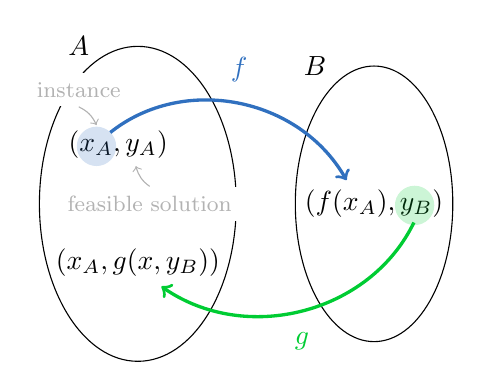
\begin{tikzpicture}[label distance=0mm,scale=1]
  \node at (-0.75,2) {$A$};
  \draw (0,0) circle[x radius=1.25,y radius=2];
  \node at (-0.25,0.75) (xA) {$(x_A,y_A)$};
  \node at (0,-0.75) (xAg) {$(x_A,g(x,y_B))$};

  \node[fill=white] at (0.15,0) (fsol) {{\color{mygrey}\footnotesize feasible solution}};
  \node[fill=white] at (-0.75,1.45) (inst) {{\color{mygrey}\footnotesize instance}};

  \path[->] (fsol.north) edge[mygrey,bend left=20] ($(xA)+(+0.225cm,-0.27cm)$);
  \path[->] (inst.south) edge[mygrey,bend left=20] ($(xA)+(-0.275cm,0.25cm)$);

  \fill[myblue,fill opacity=0.2] ($(xA)+(-0.275cm,-0.02cm)$) circle (0.25cm);

  \node at (2.25,1.75) {$B$};
  \draw (3,0) circle[x radius=1,y radius=1.75];
  \node at (3,0) (fxB) {$(f(x_A),y_B)$};

  \fill[mygreen,fill opacity=0.2] ($(fxB)+(0.515cm,-0.02cm)$) circle (0.25cm);

  \path[->] ($(xA)+(-0.1cm,0.156)$) edge[draw=myblue,very thick,bend left=50] node[label={[text=myblue]above:$f$}] {} ($(fxB.north)+(-0.35cm,0)$);
  \path[->] ($(fxB)+(0.506cm,-0.237cm)$) edge[draw=mygreen,very thick,bend left=50] node[label={[text=mygreen]below:$g$}] {} ($(xAg.south)+(0.3cm,0)$);
\end{tikzpicture}
          \end{center}
        \end{figure}
      \end{column}%
      \hfill%
      \begin{column}{.6\textwidth}
        \begin{minipage}[c][.5\textheight][c]{\linewidth}
          {\small\begin{enumerate}[(i)]
              \item $f(x_A)$ is an instance of $B$ and
                    \begin{equation*}\operatorname{OPT}(f(x_A))\leq\alpha\operatorname{OPT}(x_A)\text{,}\end{equation*}
              \item for any feasible solution $y_B$ of $f(x_A)$, $g(x_A,y_B)$ is a feasible solution of $x_A$ s.t.
                    \begin{multline*}
                      \abs{c_A(x_A,g(x_A,y_B))-\operatorname{OPT}(x_A)}\leq\\\beta\abs{c_B(f(x_A),y)-\operatorname{OPT}(f(x_A))}\text{.}
                    \end{multline*}
            \end{enumerate}}
        \end{minipage}
      \end{column}%
    \end{columns}
  \end{definition}

  \blfootnote{$\operatorname{OPT}(\cdot)$ denotes the cost of the optimal solution.}
\end{frame}

\begin{frame}
  \frametitle{L-Reduction for Metric TSP \parencite{korte_vygen_2018} I}
  \begin{columns}[T] % align columns
    \begin{column}{.35\textwidth}
      \textsc{VCP4}\footnotemark[1]
      {\footnotesize
        \begin{tabular}{ r l }
          \thead{Input:} & \makecell{undir. graph $G$ with           \\ maximum degree of 4.} \\
          \thead{Task:}  & \makecell{Find a vertex cover of $G$ with \\ minimum cardiality. }
        \end{tabular}
      }
      \begin{minipage}[c][.6\textheight][c]{\linewidth}
        \begin{figure}
          \centering
          \vspace*{0.5cm}
          \newcommand*{\vcMargin}{0.2cm}

\begin{tikzpicture}[label distance=0mm, scale=1]
  \node[graphNode,label={above:$\mathstrut u$}] (u) at (0,0) {};
  \node[graphNode,right = of u,label={above:$\mathstrut v$}] (v) {};
  \node[graphNode,below = of u,label={below:$\mathstrut w$}] (w) {};
  \node[graphNode,right = of w,label={below:$\mathstrut x$}] (x) {};
  \path[-] (u) edge (v);
  \path[-] (v) edge (w);
  \path[-] (v) edge (x);
  \path[-] (w) edge (x);

  % \filldraw[mstEdge,fill=mygreen,fill opacity=0.2] ($(v)+(\vcMargin,0)$) arc(0:180:\vcMargin)
  %   -- ($(x)+(-\vcMargin,0)$) arc(-180:0:\vcMargin)
  %   -- cycle;

  \filldraw[draw=mygreen,very thick,fill=mygreen,fill opacity=0.2] (v) to[connect=\vcMargin] (x);

  % just for positioning with G_illustration_g.tex
  \filldraw[invisible,draw=mygreen,very thick] (v) to[connect=\vcMargin] (w);

  % \node at (0.5,-2.5) (vcX) {min. VC {\color{mygreen}$X$}};
  % \path[->,mstEdge] (vcX.east) edge[bend right=50] (x.south east);

  % \node (g) at ($(x1_)!0.5!(v_)$) {Graph $G$};
\end{tikzpicture}
%
        \end{figure}
        % \begin{center}
        %   Graph $G$
        % \end{center}
      \end{minipage}
    \end{column}%
    \begin{column}{.1\textwidth}
      \vspace*{2cm}
      \begin{minipage}[c][.6\textheight][c]{\linewidth}
        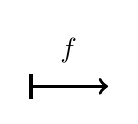
\begin{tikzpicture}[label distance=0mm, scale=1]
          \path[|->,very thick] (0,0) edge node[label={above:$\mathstrut f$}] {} (1,0);
        \end{tikzpicture}
      \end{minipage}
    \end{column}%
    \begin{column}{.55\textwidth}
      \mTSP{}
      {\footnotesize
        \begin{tabular}{ r l }
          \thead{Input:} & \makecell{undir. \& compl. graph $G$ with      \\ edge weights $c:E(G)\to\mathbb{R}_+$ that \\ satisfy the tri.-inequality.} \\
          \thead{Task:}  & \makecell{Find a Hamiltonian cycle in $G$ with \\ minimum total weight.}
        \end{tabular}
      }
      \begin{minipage}[c][.55\textheight][c]{\linewidth}
        \begin{figure}
          \centering
          \newcommand*{\edgeBend}{50}

\tikzset{
  edge4/.style={bend left=\edgeBend}
}

\begin{tikzpicture}[label distance=0mm, scale=1]
  \pic[visible on=<2->,inactiveEdges on=<3->] (wx) at (0,0) {He={\only<3->{\color{mygrey}}$\mathstrut w$}{\only<3->{\color{mygreen}}$\mathstrut x$}{}{hpStartNode on=<3->}};
  \pic[visible on=<2->,rotate=-90,inactiveEdges on=<3->] (vx) at (\HeWidth+\HeMargin,\HeWidth+\HeHeight+\HeMargin) {He={\only<3->{\color{mygreen}}$\mathstrut v$}{\only<3->{\color{mygrey}}$\mathstrut x$}{hpStartNode on=<3->}{}};
  \pic[visible on=<2->,rotate=45,inactiveEdges on=<3->] (wv) at (0.146*\HeWidth,\HeMargin+0.146*\HeWidth+\HeHeight) {He={\only<3->{\color{mygrey}}$\mathstrut w$}{\only<3->{\color{mygreen}}$\mathstrut v$}{}{hpStartNode on=<3->}};
  \pic[visible on=<2->,inactiveEdges on=<3->] (uv) at (-\HeMargin,1.146*\HeWidth+\HeHeight+3*\HeMargin) {He={\only<3->{\color{mygrey}}$\mathstrut u$}{\only<3->{\color{mygreen}}$\mathstrut v$}{}{hpStartNode on=<3->}};

  \begin{scope}[on background layer]
    \draw[visible on=<4->,inactiveEdges on=<5->] (uv-v1) edge[edge4] (wv-v1);
    \draw[visible on=<4->,inactiveEdges on=<5->] (uv-v1) edge[edge4] (wv-v2);
    \draw[visible on=<4->,inactiveEdges on=<5->] (uv-v2) edge[edge4] (wv-v1);
    \draw[visible on=<4->,inactiveEdges on=<5->] (uv-v2) edge[edge4] (wv-v2);

    \draw[visible on=<4->,inactiveEdges on=<5->] (uv-v1) edge[edge4] (vx-u1);
    \draw[visible on=<4->,inactiveEdges on=<5->] (uv-v1) edge[edge4] (vx-u2);
    \draw[visible on=<4->,inactiveEdges on=<5->] (uv-v2) edge[edge4] (vx-u1);
    \draw[visible on=<4->,inactiveEdges on=<5->] (uv-v2) edge[edge4] (vx-u2);

    \draw[visible on=<4->,inactiveEdges on=<5->] (wv-v1) edge[edge4] (vx-u1);
    \draw[visible on=<4->,inactiveEdges on=<5->] (wv-v1) edge[edge4] (vx-u2);
    \draw[visible on=<4->,inactiveEdges on=<5->] (wv-v2) edge[edge4] (vx-u1);
    \draw[visible on=<4->,inactiveEdges on=<5->] (wv-v2) edge[edge4] (vx-u2);

    \draw[visible on=<4->,inactiveEdges on=<5->] (wx-u1) edge[edge4] (wv-u1);
    \draw[visible on=<4->,inactiveEdges on=<5->] (wx-u1) edge[edge4] (wv-u2);
    \draw[visible on=<4->,inactiveEdges on=<5->] (wx-u2) edge[edge4] (wv-u1);
    \draw[visible on=<4->,inactiveEdges on=<5->] (wx-u2) edge[edge4] (wv-u2);

    \draw[visible on=<4->,inactiveEdges on=<5->] (vx-v1) edge[edge4] (wx-v1);
    \draw[visible on=<4->,inactiveEdges on=<5->] (vx-v1) edge[edge4] (wx-v2);
    \draw[visible on=<4->,inactiveEdges on=<5->] (vx-v2) edge[edge4] (wx-v1);
    \draw[visible on=<4->,inactiveEdges on=<5->] (vx-v2) edge[edge4] (wx-v2);
  \end{scope}

  \draw[visible on=<3->,lr1Edge] (uv-v1) -- (uv-v3) -- (uv-u2) -- (uv-v5)
  -- (uv-u6) -- (uv-v4) -- (uv-u5) -- (uv-v6) -- (uv-u4)
  -- (uv-u1) -- (uv-u3) -- (uv-v2);

  \draw[visible on=<3->,lr1Edge] (wv-v1) -- (wv-v3) -- (wv-u2) -- (wv-v5)
  -- (wv-u6) -- (wv-v4) -- (wv-u5) -- (wv-v6) -- (wv-u4)
  -- (wv-u1) -- (wv-u3) -- (wv-v2);

  \draw[visible on=<3->,lr1Edge] (vx-u1) -- (vx-u3) -- (vx-v2) -- (vx-u5)
  -- (vx-v6) -- (vx-u4) -- (vx-v5) -- (vx-u6) -- (vx-v4)
  -- (vx-v1) -- (vx-v3) -- (vx-u2);

  \draw[visible on=<3->,lr1Edge] (wx-v1) -- (wx-v3) -- (wx-u2) -- (wx-v5)
  -- (wx-u6) -- (wx-v4) -- (wx-u5) -- (wx-v6) -- (wx-u4)
  -- (wx-u1) -- node[lr1EdgeLabel] {\footnotesize 1} (wx-u3) -- (wx-v2);

  \draw[visible on=<5->,lr4Edge] (uv-v1) edge[edge4] (wv-v2);
  \draw[visible on=<5->,lr4Edge] (wv-v1) edge[edge4] node[lr4EdgeLabel] {} (vx-u2);
  
  \draw[visible on=<6->,lr5Edge] (wx-v1)
  .. controls ++(2*\HeWidth,-\HeMargin) and ++(2*\HeWidth,\HeMargin) .. node[lr5EdgeLabel] {\footnotesize 5}
  (uv-v2);

  \draw[visible on=<6->,lr5Edge] (wx-v2)
  .. controls ++(\HeHeight,-\HeHeight) and ++(\HeHeight,-\HeHeight) ..
  (vx-u1);

  % just for positioning with H_illustration_g.tex
  \draw[invisible,lr5Edge] (wv-u1)
  .. controls ++(-2*\HeMargin,2*\HeMargin) and ++(-\HeWidth-2*\HeMargin,\HeHeight+\HeMargin) .. node[lr5EdgeLabel] {\footnotesize 5}
  (uv-v2);

  \draw[invisible,lr5Edge] (wx-u2)
  .. controls ++(\HeWidth+\HeMargin,-\HeHeight) and ++(\HeHeight,-\HeWidth-\HeMargin) ..
  (vx-u1);

  \node[align=left] at ($(vx-u1 |- uv-v2)+(0.25,0)$) {\tiny\shortstack[l]{*Not all edges \\ \tiny are shown.}};

\end{tikzpicture}
        \end{figure}
      \end{minipage}
      % \begin{center}
      %   Graph $H:=f(G)$
      % \end{center}
    \end{column}%
  \end{columns}

  \footnotetext[1]{\textsc{Minimum Vertex Cover Problem} with maximum degree of 4}
\end{frame}

\begin{frame}
  \frametitle{L-Reduction for Metric TSP \parencite{korte_vygen_2018} II}
  \begin{columns}[T] % align columns
    \begin{column}{.35\textwidth}
      \textsc{VCP4}\footnotemark[1]
      {\footnotesize
        \begin{tabular}{ r l }
          \thead{Input:} & \makecell{undir. graph $G$ with           \\ maximum degree of 4.} \\
          \thead{Task:}  & \makecell{Find a vertex cover of $G$ with \\ minimum cardiality. }
        \end{tabular}
      }
      \begin{minipage}[c][.6\textheight][c]{\linewidth}
        \begin{figure}
          \centering
          \vspace*{0.5cm}
          \newcommand*{\vcMargin}{0.2cm}

\begin{tikzpicture}[label distance=0mm, scale=1]
  \node[graphNode,label={above:$\mathstrut u$}] (u) at (0,0) {};
  \node[graphNode,right = of u,label={above:$\mathstrut v$}] (v) {};
  \node[graphNode,below = of u,label={below:$\mathstrut w$}] (w) {};
  \node[graphNode,right = of w,label={below:$\mathstrut x$}] (x) {};
  \path[-] (u) edge (v);
  \path[-] (v) edge (w);
  \path[-] (v) edge (x);
  \path[-] (w) edge (x);

  % \filldraw[mstEdge,fill=mygreen,fill opacity=0.2] ($(v)+(\vcMargin,0)$) arc(0:180:\vcMargin)
  %   -- ($(x)+(-\vcMargin,0)$) arc(-180:0:\vcMargin)
  %   -- cycle;

  \filldraw[draw=mygreen,very thick,fill=mygreen,fill opacity=0.2,visible on=<3->] (v) to[connect=\vcMargin] (w);

  % just for positioning with G_illustration_f.tex
  \filldraw[invisible,draw=mygreen,very thick] (v) to[connect=\vcMargin] (x);

  % \node at (0.5,-2.5) (vcX) {min. VC {\color{mygreen}$X$}};
  % \path[->,mstEdge] (vcX.east) edge[bend right=50] (x.south east);

  % \node (g) at ($(x1_)!0.5!(v_)$) {Graph $G$};
\end{tikzpicture}
%
        \end{figure}
        % \begin{center}
        %   Graph $G$
        % \end{center}
      \end{minipage}
    \end{column}%
    \begin{column}{.1\textwidth}
      \vspace*{2cm}
      \begin{minipage}[c][.6\textheight][c]{\linewidth}
        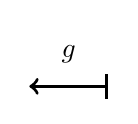
\begin{tikzpicture}[label distance=0mm, scale=1]
          \path[<-|,very thick] (0,0) edge node[label={above:$\mathstrut g$}] {} (1,0);
        \end{tikzpicture}
      \end{minipage}
    \end{column}%
    \begin{column}{.55\textwidth}
      \mTSP{}
      {\footnotesize
        \begin{tabular}{ r l }
          \thead{Input:} & \makecell{undir. \& compl. graph $G$ with      \\ edge weights $c:E(G)\to\mathbb{R}_+$ that \\ satisfy the tri.-inequality.} \\
          \thead{Task:}  & \makecell{Find a Hamiltonian cycle in $G$ with \\ minimum total weight.}
        \end{tabular}
      }
      \begin{minipage}[c][.55\textheight][c]{\linewidth}
        \begin{figure}
          \centering
          \newcommand*{\edgeBend}{50}

\tikzset{
  edge4/.style={bend left=\edgeBend}
}

\begin{tikzpicture}[label distance=0mm, scale=1]
  \pic[inactiveEdges on=<1->] (wx) at (0,0) {He={\only<3->{\color{mygreen}}$\mathstrut w$}{\only<3->{\color{mygrey}}$\mathstrut x$}{hpStartNode on=<3->}{}};
  \pic[rotate=-90,inactiveEdges on=<1->] (vx) at (\HeWidth+\HeMargin,\HeWidth+\HeHeight+\HeMargin) {He={\only<3->{\color{mygreen}}$\mathstrut v$}{\only<3->{\color{mygrey}}$\mathstrut x$}{hpStartNode on=<3->}{}};
  \pic[rotate=45,inactiveEdges on=<1->] (wv) at (0.146*\HeWidth,\HeMargin+0.146*\HeWidth+\HeHeight) {He={\only<3->{\color{mygreen}}$\mathstrut w$}{\only<3->{\color{mygrey}}$\mathstrut v$}{hpStartNode on=<3->}{}};
  \pic[inactiveEdges on=<1->] (uv) at (-\HeMargin,1.146*\HeWidth+\HeHeight+3*\HeMargin) {He={\only<3->{\color{mygrey}}$\mathstrut u$}{\only<3->{\color{mygreen}}$\mathstrut v$}{}{hpStartNode on=<3->}};

  \begin{scope}[on background layer]
    \draw[inactiveEdge] (uv-v1) edge[edge4] (wv-v1);
    \draw[inactiveEdge] (uv-v1) edge[edge4] (wv-v2);
    \draw[inactiveEdge] (uv-v2) edge[edge4] (wv-v1);
    \draw[inactiveEdge] (uv-v2) edge[edge4] (wv-v2);

    \draw[inactiveEdge] (uv-v1) edge[edge4] (vx-u1);
    \draw[inactiveEdge] (uv-v1) edge[edge4] (vx-u2);
    \draw[inactiveEdge] (uv-v2) edge[edge4] (vx-u1);
    \draw[inactiveEdge] (uv-v2) edge[edge4] (vx-u2);

    \draw[inactiveEdge] (wv-v1) edge[edge4] (vx-u1);
    \draw[inactiveEdge] (wv-v1) edge[edge4] (vx-u2);
    \draw[inactiveEdge] (wv-v2) edge[edge4] (vx-u1);
    \draw[inactiveEdge] (wv-v2) edge[edge4] (vx-u2);

    \draw[inactiveEdge] (wx-u1) edge[edge4] (wv-u1);
    \draw[inactiveEdge] (wx-u1) edge[edge4] (wv-u2);
    \draw[inactiveEdge] (wx-u2) edge[edge4] (wv-u1);
    \draw[inactiveEdge] (wx-u2) edge[edge4] (wv-u2);

    \draw[inactiveEdge] (vx-v1) edge[edge4] (wx-v1);
    \draw[inactiveEdge] (vx-v1) edge[edge4] (wx-v2);
    \draw[inactiveEdge] (vx-v2) edge[edge4] (wx-v1);
    \draw[inactiveEdge] (vx-v2) edge[edge4] (wx-v2);
  \end{scope}

  \draw[lrRandomEdge on=<1-3>,lr1Edge on=<3->] (uv-v1) -- (uv-v3) -- (uv-u2) -- (uv-v5)
  -- (uv-u6) -- (uv-v4) -- (uv-u5) -- (uv-v6) -- (uv-u4)
  -- (uv-u1) -- (uv-u3) -- (uv-v2);

  \draw[lrRandomEdge on=<1-3>,lr1Edge on=<3->] (wv-u1) -- (wv-u3) -- (wv-v2) -- (wv-u5)
  -- (wv-v6) -- (wv-u4) -- (wv-v5) -- (wv-u6) -- (wv-v4)
  -- (wv-v1) -- (wv-v3) -- (wv-u2);

  \draw[lrRandomEdge,invisible on=<2->] (vx-u2) -- (vx-v5) -- (vx-u4) -- (vx-u1)
  -- (vx-u3) -- (vx-v2)
  -- (wx-v4) -- (wx-u5) -- (wx-v6) -- (wx-u6) -- (wx-v1) -- (wx-v3) -- (wx-u4) -- (wx-v2)
  -- (vx-v3) -- (vx-u6) -- (vx-v6) -- (vx-u5) -- (vx-v4) -- (vx-v1)
  -- (wx-u1) -- (wx-u3) -- (wx-u2) -- (wx-v5);

  \draw[lrRandomEdge,invisible on=<2->] (wx-v5) edge[edge4] (wv-u2);

  \draw[visible on=<2->,lr1Edge] (vx-u1) -- (vx-u3) -- (vx-v2) -- (vx-u5)
  -- (vx-v6) -- (vx-u4) -- (vx-v5) -- (vx-u6) -- (vx-v4)
  -- (vx-v1) -- (vx-v3) -- (vx-u2);

  \draw[visible on=<2->,lr1Edge] (wx-u1) -- node[visible on=<2->,lr1EdgeLabel] {\footnotesize 1} (wx-u3) -- (wx-v2) -- (wx-u5)
  -- (wx-v6) -- (wx-u4) -- (wx-v5) -- (wx-u6) -- (wx-v4)
  -- (wx-v1) -- (wx-v3) -- (wx-u2);

  \draw[visible on=<2->,lr4Edge on=<2->] (wx-u1) edge[edge4] (wv-u2);
  \draw[lrRandomEdge on=<1-2>,lr4Edge on=<2->] (uv-v1) edge[edge4,text visible on=<2->] node[lr4EdgeLabel] {} (vx-u2);

  \draw[lrRandomEdge on=<1-3>,lr5Edge on=<3->] (wv-u1)
  .. controls ++(-2*\HeMargin,2*\HeMargin) and ++(-\HeWidth-2*\HeMargin,\HeHeight+\HeMargin) ..
  (uv-v2);

  \draw[visible on=<2->,lrRandomEdge on=<1-2>,lr5Edge on=<2->] (wx-u2)
  .. controls ++(\HeWidth+\HeMargin,-\HeHeight) and ++(\HeHeight,-\HeWidth-\HeMargin) .. node[visible on=<2->,lr5EdgeLabel] {\footnotesize 5}
  (vx-u1);

  % just for positioning with H_illustration_f.tex
  \draw[invisible,lr5Edge] (wx-v1)
  .. controls ++(2*\HeWidth,-\HeMargin) and ++(2*\HeWidth,\HeMargin) .. node[visible on=<2->,lr5EdgeLabel] {\footnotesize 5}
  (uv-v2);

  \draw[invisible,lr5Edge] (wx-v2)
  .. controls ++(\HeHeight,-\HeHeight) and ++(\HeHeight,-\HeHeight) ..
  (vx-u1);

  \node[align=left] at ($(vx-u1 |- uv-v2)+(0.25,0)$) {\tiny\shortstack[l]{*Not all edges \\ \tiny are shown.}};

\end{tikzpicture}
        \end{figure}
      \end{minipage}
      % \begin{center}
      %   Graph $H:=f(G)$
      % \end{center}
    \end{column}%
  \end{columns}
  \footnotetext[1]{\textsc{Minimum Vertex Cover Problem} with maximum degree of 4}
\end{frame}

\begin{frame}
  \frametitle{Formalization of L-Reduction for Metric TSP}

  I have formalized the L-reduction in Isabelle/HOL. % \parencite{nipkow_wenzel_paulson_2002}.

  \begin{itemize}
    \item A locale provides an abstract executable graph representation based on an adjacency map.
    \item The locale assumes \texttt{fold}-functions to do computation on the graphs.
          \begin{itemize}
            \item This approach is adapted from \parencite{abdulaziz_2022}.
          \end{itemize}
    \item Abstract versions of the reduction functions $f$ and $g$ are defined using the \texttt{fold}-functions.
    \item The feasibility of the function $f$ and $g$ and the linear inequalities are proven.
    \item The locale is instantiated with concrete implementations to obtain executable versions of the functions $f$ and $g$.
  \end{itemize}
  \vspace*{0.5cm}
  \pause
  {\color{myred} The L-reduction in \parencite[Thm. 21.6,][]{korte_vygen_2018} is incomplete.}
  \begin{enumerate}[(i)]
    \item The proof for the linear inequalities fails if the optimal vertex cover has a cardinality of 1.
    \item Not all cases are covered when constructing a vertex cover from a Hamiltonian cycle.
  \end{enumerate}
\end{frame}

\begin{frame}
  \frametitle{Conclusion and Future Work}

  \begin{itemize}
    \item I have formally verified two approx. algorithms for \mTSP{}.
    \item I have formalized a L-reduction from \textsc{VCP4}\footnotemark[1]{} to \mTSP{}, which proves the \maxSNP{}-hardness of \mTSP{}.
  \end{itemize}
  \vspace*{0.5cm}
  \pause
  \begin{itemize}
    \item Prove the existence of the necessary algorithms for the \textsc{Christofides-Serdyukov} algorithm.
          \begin{itemize}
            \item Write an adaptor to the existing formalization of Prim's algorithm \parencite{lammich_nipkow_2019}.
            \item Formalize and verify algorithms for minimum perfect-matching and Eulerian tour \parencite[Sec. 11.2 \& 2.4,][]{korte_vygen_2018}.
          \end{itemize}
    \item Formalize an encoding of multigraphs with simple graphs.
    \item Prove the polynomial running time of reduction functions $f$ and $g$.
          \begin{itemize}
            \item Refine the functions $f$ and $g$ to \texttt{IMP-} and prove their running time.
          \end{itemize}
  \end{itemize}
  \footnotetext[1]{\textsc{Minimum Vertex Cover Problem} with maximum degree of 4}
\end{frame}

\begin{frame}[allowframebreaks]{References}
  \printbibliography
\end{frame}

\appendix
\backupbegin

\begin{frame}
  \frametitle{Appendix -- Equiv. Max. Matching and Min. Matching}

  Let $G$ be an undirected graph with edge weights $c$.
  \vspace*{0.25cm}
  \begin{enumerate}[(i)]
    \item \textsc{MaxMatch}\footnotemark[1]{} solves \textsc{MinMatch}\footnotemark[2]{}. Assume $f$ solves \textsc{MaxMatch}.
  \end{enumerate}
  \begin{equation*}
    c'(e) := 1 + - c(e) + \sum_{e'\in E(G)} c(e')
  \end{equation*}
  \vspace*{-0.4cm}
  \begin{itemize}
    \item If matching $M:=f(G,c')$ is perfect return $M$ otherwise None.
  \end{itemize}
  \vspace*{0.5cm}
  \begin{enumerate}[(i)]
    \setcounter{enumi}{1}
    \item \textsc{MinMatch} solves \textsc{MaxMatch}. Assume $f$ solves \textsc{MinMatch}.
  \end{enumerate}
  \vspace*{-0.25cm}
  \begin{align*}
    E_1 & := \left\{e\times\{1\}\mid e\in E(G)\right\} & E_2 & := \left\{e\times\{2\}\mid e\in E(G)\right\}
  \end{align*}
  \vspace*{-1cm}
  \begin{align*}
    E_V & := \left\{\{(v,1),(v,2)\}\mid v\in V(G)\right\}
  \end{align*}
  \vspace*{-1cm}
  \begin{align*}
    H & := \left(V(G)\times\{1,2\},E_1\cup E_2\cup E_V\right) & c'(e) & := \begin{cases*} 1 & if $e\in E_V$ \\ -c(e) & otherwise\end{cases*}
  \end{align*}
  \vspace*{-0.4cm}
  \begin{itemize}
    \item Return matching $M:=f(H,c')\cap E_1$.
  \end{itemize}

  \footnotetext[1]{\textsc{Maximum Matching Problem}}
  \footnotetext[2]{\textsc{Minimum Matching-Perfect Problem}}
\end{frame}

\begin{frame}
  \frametitle{Appendix -- Approximation Algorithms for Metric TSP}

  Let $(G,c)$ be an instance of \mTSP{}.

  \begin{lemma}[21.3, \cite{korte_vygen_2018}]
    Given a connected Eulerian graph $G'$ that spans $V(G)$, we can compute (in polynomial time) a Hamiltonian cycle for $G$ with total weight of at most $c(E(G'))$.
  \end{lemma}
  \begin{proofIdea}
    \begin{enumerate}
      \item Compute a Eulerian tour in $G'$.
      \item Remove duplicate vertices ("shortcutting").
    \end{enumerate}
  \end{proofIdea}

  \begin{itemize}
    \item[$\implies$] We only need to find Eulerian graph that spans $V(G)$ with the smallest total weight!
  \end{itemize}
\end{frame}

\begin{frame}
  \frametitle{Appendix -- DoubleTree Algorithm}

  \begin{theorem}[21.4, \cite{korte_vygen_2018}]
    \textsc{DoubleTree} is a 2-approximation algorithm for \mTSP{}.
  \end{theorem}
  % \begin{proofIdea}
  %   The total weight of any Hamiltonian cycle is at least the total weight of a MST.
  % \end{proofIdea}

  \begin{columns}[T] % align columns
    \begin{column}{.35\textwidth}
      \begin{figure}
        % \begin{overprint}
        %   \onslide<1>\begin{center}\newcommand*{\circleDia}{2.0cm}
\newcommand*{\edgeBend}{0}
\newcommand*{\etMargin}{0.15cm}

\begin{tikzpicture}[label distance=0mm,scale=1]
  \foreach \a in {1,2,...,5}{
      \draw (90+144-\a*360/5: \circleDia) node[graphNode,label={90+144-\a*360/5:$\mathstrut \a$}] (\a) {};
    }

  % \draw[white,name path=line21] ($(2)!-\etMargin!(1)!-\etMargin!90:(1)$) -- ($(1)!-\etMargin!(2)!\etMargin!90:(2)$);
  % \draw[white,name path=line32] ($(3)!-\etMargin!(2)!-\etMargin!90:(2)$) -- ($(2)!-\etMargin!(3)!-\etMargin!-90:(3)$);
  % \draw[white,name path=line12] ($(1)!-\etMargin!(2)!-\etMargin!90:(2)$) -- ($(2)!-\etMargin!(1)!-\etMargin!-90:(1)$);
  % \draw[white,name path=line25] ($(2)!-\etMargin!(5)!-\etMargin!90:(5)$) -- ($(5)!-\etMargin!(2)!\etMargin!90:(2)$);
  % \draw[white,name path=line45] ($(4)!-\etMargin!(5)!-\etMargin!90:(5)$) -- ($(5)!-\etMargin!(4)!-\etMargin!-90:(4)$);
  % \draw[white,name path=line52] ($(5)!-\etMargin!(2)!-\etMargin!90:(2)$) -- ($(2)!-\etMargin!(5)!-\etMargin!-90:(5)$);
  % \draw[white,name path=line23] ($(2)!-\etMargin!(3)!-\etMargin!90:(3)$) -- ($(3)!-\etMargin!(2)!\etMargin!90:(2)$);

  % \path [name intersections={of=line21 and line32,by=line123}];
  % \path [name intersections={of=line12 and line25,by=line125}];
  % \path [name intersections={of=line45 and line52,by=line452}];
  % \path [name intersections={of=line52 and line23,by=line523}];

  \path[-] (1) edge node[edgeLabel] {\footnotesize $2$} (2);
  % \path[-] (1) edge[mstEdge,bend right=\edgeBend] node[mstEdgeLabel] {\footnotesize $2$} (2);
  % \path[-] (1) edge[mstEdge,bend left=\edgeBend] node[mstEdgeLabel] {\footnotesize $2$} (2);
  \path[-] (1) edge node[edgeLabel] {\footnotesize $3$} (3);
  \path[-] (1) edge node[edgeLabel] {\footnotesize $3$} (4);
  \path[-] (1) edge node[edgeLabel] {\footnotesize $3$} (5);

  \path[-] (2) edge node[edgeLabel] {\footnotesize $2$} (3);
  % \path[-] (2) edge[mstEdge,bend right=\edgeBend] node[mstEdgeLabel] {\footnotesize $2$} (3);
  % \path[-] (2) edge[mstEdge,bend left=\edgeBend] node[mstEdgeLabel] {\footnotesize $2$} (3);
  \path[-] (2) edge node[edgeLabel] {\footnotesize $3$} (4);
  \path[-] (2) edge node[edgeLabel] {\footnotesize $1$} (5);
  % \path[-] (2) edge[mstEdge,bend right=\edgeBend] node[mstEdgeLabel] {\footnotesize $1$} (5);
  % \path[-] (2) edge[mstEdge,bend left=\edgeBend] node[mstEdgeLabel] {\footnotesize $1$} (5);

  \path[-] (3) edge node[edgeLabel] {\footnotesize $3$} (4);
  \path[-] (3) edge node[edgeLabel] {\footnotesize $2$} (5);

  \path[-] (4) edge node[edgeLabel] {\footnotesize $2$} (5);
  % \path[-] (4) edge[mstEdge,bend right=\edgeBend] node[mstEdgeLabel] {\footnotesize $2$} (5);
  % \path[-] (4) edge[mstEdge,bend left=\edgeBend] node[mstEdgeLabel] {\footnotesize $2$} (5);

  % \draw[blue!50,very thick,rounded corners=\etMargin] (line123) -- ($(1)!-\etMargin!(2)!\etMargin!90:(2)$)
  % -- ($(1)!-\etMargin!(2)!-\etMargin!90:(2)$) -- (line125)
  % -- ($(5)!-\etMargin!(2)!\etMargin!90:(2)$)
  % -- ($(5)!-\etMargin!(4)!-\etMargin!90:(4)$) -- ($(4)!-\etMargin!(5)!\etMargin!90:(5)$)
  % -- ($(4)!-\etMargin!(5)!-\etMargin!90:(5)$) -- (line452)
  % -- (line523)
  % -- ($(3)!-\etMargin!(2)!\etMargin!90:(2)$)
  % -- ($(3)!-\etMargin!(2)!-\etMargin!90:(2)$) -- cycle;

\end{tikzpicture}
\end{center}
        %   \onslide<2>\begin{center}\newcommand*{\circleDia}{2.0cm}
\newcommand*{\edgeBend}{0}

\begin{tikzpicture}[label distance=0mm,scale=1]
  \foreach \a in {1,2,...,5}{
      \draw (90+144-\a*360/5: \circleDia) node[graphNode,label={90+144-\a*360/5:$\mathstrut \a$}] (\a) {};
    }

  % \path[-] (1) edge node[edgeLabel] {\footnotesize $2$} (2);
  \path[-] (1) edge[mstEdge,bend right=\edgeBend] node[mstEdgeLabel] {\footnotesize $2$} (2);
  % \path[-] (1) edge[mstEdge,bend left=\edgeBend] node[mstEdgeLabel] {\footnotesize $2$} (2);
  \path[-] (1) edge[inactiveEdge] node[inactiveEdgeLabel] {\footnotesize $3$} (3);
  \path[-] (1) edge[inactiveEdge] node[inactiveEdgeLabel] {\footnotesize $3$} (4);
  \path[-] (1) edge[inactiveEdge] node[inactiveEdgeLabel] {\footnotesize $3$} (5);

  % \path[-] (2) edge node[edgeLabel] {\footnotesize $2$} (3);
  \path[-] (2) edge[mstEdge,bend right=\edgeBend] node[mstEdgeLabel] {\footnotesize $2$} (3);
  % \path[-] (2) edge[mstEdge,bend left=\edgeBend] node[mstEdgeLabel] {\footnotesize $2$} (3);
  \path[-] (2) edge[inactiveEdge] node[inactiveEdgeLabel] {\footnotesize $3$} (4);
  % \path[-] (2) edge node[edgeLabel] {\footnotesize $1$} (5);
  \path[-] (2) edge[mstEdge,bend right=\edgeBend] node[mstEdgeLabel] {\footnotesize $1$} (5);
  % \path[-] (2) edge[mstEdge,bend left=\edgeBend] node[mstEdgeLabel] {\footnotesize $1$} (5);

  \path[-] (3) edge[inactiveEdge] node[inactiveEdgeLabel] {\footnotesize $3$} (4);
  \path[-] (3) edge[inactiveEdge] node[inactiveEdgeLabel] {\footnotesize $2$} (5);

  % \path[-] (4) edge node[edgeLabel] {\footnotesize $2$} (5);
  \path[-] (4) edge[mstEdge,bend right=\edgeBend] node[mstEdgeLabel] {\footnotesize $2$} (5);
  % \path[-] (4) edge[mstEdge,bend left=\edgeBend] node[mstEdgeLabel] {\footnotesize $2$} (5);

\end{tikzpicture}
\end{center}
        %   \onslide<3>\begin{center}\newcommand*{\circleDia}{2.0cm}
\newcommand*{\edgeBend}{15}

\begin{tikzpicture}[label distance=0mm,scale=1]
  \foreach \a in {1,2,...,5}{
      \draw (90+144-\a*360/5: \circleDia) node[graphNode,label={90+144-\a*360/5:$\mathstrut \a$}] (\a) {};
    }

  % \path[-] (1) edge node[edgeLabel] {\footnotesize $2$} (2);
  \path[-] (1) edge[mstEdge,bend right=\edgeBend] node[mstEdgeLabel] {\footnotesize $2$} (2);
  \path[-] (1) edge[mstEdge,bend left=\edgeBend] node[mstEdgeLabel] {\footnotesize $2$} (2);
  \path[-] (1) edge[inactiveEdge] node[inactiveEdgeLabel] {\footnotesize $3$} (3);
  \path[-] (1) edge[inactiveEdge] node[inactiveEdgeLabel] {\footnotesize $3$} (4);
  \path[-] (1) edge[inactiveEdge] node[inactiveEdgeLabel] {\footnotesize $3$} (5);

  % \path[-] (2) edge node[edgeLabel] {\footnotesize $2$} (3);
  \path[-] (2) edge[mstEdge,bend right=\edgeBend] node[mstEdgeLabel] {\footnotesize $2$} (3);
  \path[-] (2) edge[mstEdge,bend left=\edgeBend] node[mstEdgeLabel] {\footnotesize $2$} (3);
  \path[-] (2) edge[inactiveEdge] node[inactiveEdgeLabel] {\footnotesize $3$} (4);
  % \path[-] (2) edge node[edgeLabel] {\footnotesize $1$} (5);
  \path[-] (2) edge[mstEdge,bend right=\edgeBend] node[mstEdgeLabel] {\footnotesize $1$} (5);
  \path[-] (2) edge[mstEdge,bend left=\edgeBend] node[mstEdgeLabel] {\footnotesize $1$} (5);

  \path[-] (3) edge[inactiveEdge] node[inactiveEdgeLabel] {\footnotesize $3$} (4);
  \path[-] (3) edge[inactiveEdge] node[inactiveEdgeLabel] {\footnotesize $2$} (5);

  % \path[-] (4) edge node[edgeLabel] {\footnotesize $2$} (5);
  \path[-] (4) edge[mstEdge,bend right=\edgeBend] node[mstEdgeLabel] {\footnotesize $2$} (5);
  \path[-] (4) edge[mstEdge,bend left=\edgeBend] node[mstEdgeLabel] {\footnotesize $2$} (5);

\end{tikzpicture}
\end{center}
        %   \onslide<4>\begin{center}\newcommand*{\circleDia}{2.0cm}
\newcommand*{\edgeBend}{15}

\begin{tikzpicture}[label distance=0mm,scale=1]
  \foreach \a in {1,2,...,5}{
      \draw (90+144-\a*360/5: \circleDia) node[graphNode,label={90+144-\a*360/5:$\mathstrut \a$}] (\a) {};
    }

  % \path[-] (1) edge node[edgeLabel] {\footnotesize $2$} (2);
  \path[-] (1) edge[mstEdge,bend right=\edgeBend] node[mstEdgeLabel] {\footnotesize $2$} (2);
  \path[-] (1) edge[mstEdge,bend left=\edgeBend] node[mstEdgeLabel] {\footnotesize $2$} (2);
  \path[-] (1) edge[inactiveEdge] node[inactiveEdgeLabel] {\footnotesize $3$} (3);
  \path[-] (1) edge[inactiveEdge] node[inactiveEdgeLabel] {\footnotesize $3$} (4);
  \path[-] (1) edge[inactiveEdge] node[inactiveEdgeLabel] {\footnotesize $3$} (5);

  % \path[-] (2) edge node[edgeLabel] {\footnotesize $2$} (3);
  \path[-] (2) edge[mstEdge,bend right=\edgeBend] node[mstEdgeLabel] {\footnotesize $2$} (3);
  \path[-] (2) edge[mstEdge,bend left=\edgeBend] node[mstEdgeLabel] {\footnotesize $2$} (3);
  \path[-] (2) edge[inactiveEdge] node[inactiveEdgeLabel] {\footnotesize $3$} (4);
  % \path[-] (2) edge node[edgeLabel] {\footnotesize $1$} (5);
  \path[-] (2) edge[mstEdge,bend right=\edgeBend] node[mstEdgeLabel] {\footnotesize $1$} (5);
  \path[-] (2) edge[mstEdge,bend left=\edgeBend] node[mstEdgeLabel] {\footnotesize $1$} (5);

  \path[-] (3) edge[inactiveEdge] node[inactiveEdgeLabel] {\footnotesize $3$} (4);
  \path[-] (3) edge[inactiveEdge] node[inactiveEdgeLabel] {\footnotesize $2$} (5);

  % \path[-] (4) edge node[edgeLabel] {\footnotesize $2$} (5);
  \path[-] (4) edge[mstEdge,bend right=\edgeBend] node[mstEdgeLabel] {\footnotesize $2$} (5);
  \path[-] (4) edge[mstEdge,bend left=\edgeBend] node[mstEdgeLabel] {\footnotesize $2$} (5);

  \node[circle,fill=myred,inner sep=0.05cm] at (2) {};

\end{tikzpicture}
\end{center}
        %   \onslide<5>\begin{center}\newcommand*{\circleDia}{2.0cm}
\newcommand*{\edgeBend}{15}

\begin{tikzpicture}[label distance=0mm,scale=1]
  \foreach \a in {1,2,...,5}{
      \draw (90+144-\a*360/5: \circleDia) node[graphNode,label={90+144-\a*360/5:$\mathstrut \a$}] (\a) {};
    }

  % \path[-] (1) edge node[edgeLabel] {\footnotesize $2$} (2);
  \path[-] (1) edge[mstEdge,bend right=\edgeBend] node[mstEdgeLabel] {\footnotesize $2$} (2);
  \path[-] (1) edge[resultEdge,bend left=\edgeBend] node[resultEdgeLabel] {\footnotesize $2$} (2);
  \path[-] (1) edge[inactiveEdge] node[inactiveEdgeLabel] {\footnotesize $3$} (3);
  \path[-] (1) edge[inactiveEdge] node[inactiveEdgeLabel] {\footnotesize $3$} (4);
  \path[-] (1) edge[inactiveEdge] node[inactiveEdgeLabel] {\footnotesize $3$} (5);

  % \path[-] (2) edge node[edgeLabel] {\footnotesize $2$} (3);
  \path[-] (2) edge[mstEdge,bend right=\edgeBend] node[mstEdgeLabel] {\footnotesize $2$} (3);
  \path[-] (2) edge[mstEdge,bend left=\edgeBend] node[mstEdgeLabel] {\footnotesize $2$} (3);
  \path[-] (2) edge[inactiveEdge] node[inactiveEdgeLabel] {\footnotesize $3$} (4);
  % \path[-] (2) edge node[edgeLabel] {\footnotesize $1$} (5);
  \path[-] (2) edge[mstEdge,bend right=\edgeBend] node[mstEdgeLabel] {\footnotesize $1$} (5);
  \path[-] (2) edge[mstEdge,bend left=\edgeBend] node[mstEdgeLabel] {\footnotesize $1$} (5);

  \path[-] (3) edge[inactiveEdge] node[inactiveEdgeLabel] {\footnotesize $3$} (4);
  \path[-] (3) edge[inactiveEdge] node[inactiveEdgeLabel] {\footnotesize $2$} (5);

  % \path[-] (4) edge node[edgeLabel] {\footnotesize $2$} (5);
  \path[-] (4) edge[mstEdge,bend right=\edgeBend] node[mstEdgeLabel] {\footnotesize $2$} (5);
  \path[-] (4) edge[mstEdge,bend left=\edgeBend] node[mstEdgeLabel] {\footnotesize $2$} (5);

  \node[circle,fill=myred,inner sep=0.05cm] at (1) {};

\end{tikzpicture}
\end{center}
        %   \onslide<6>\begin{center}\newcommand*{\circleDia}{2.0cm}
\newcommand*{\edgeBend}{15}

\begin{tikzpicture}[label distance=0mm,scale=1]
  \foreach \a in {1,2,...,5}{
      \draw (90+144-\a*360/5: \circleDia) node[graphNode,label={90+144-\a*360/5:$\mathstrut \a$}] (\a) {};
    }

  % \path[-] (1) edge node[edgeLabel] {\footnotesize $2$} (2);
  \path[-] (1) edge[resultEdge,bend right=\edgeBend] node[resultEdgeLabel] {\footnotesize $2$} (2);
  \path[-] (1) edge[resultEdge,bend left=\edgeBend] node[resultEdgeLabel] {\footnotesize $2$} (2);
  \path[-] (1) edge[inactiveEdge] node[inactiveEdgeLabel] {\footnotesize $3$} (3);
  \path[-] (1) edge[inactiveEdge] node[inactiveEdgeLabel] {\footnotesize $3$} (4);
  \path[-] (1) edge[inactiveEdge] node[inactiveEdgeLabel] {\footnotesize $3$} (5);

  % \path[-] (2) edge node[edgeLabel] {\footnotesize $2$} (3);
  \path[-] (2) edge[mstEdge,bend right=\edgeBend] node[mstEdgeLabel] {\footnotesize $2$} (3);
  \path[-] (2) edge[mstEdge,bend left=\edgeBend] node[mstEdgeLabel] {\footnotesize $2$} (3);
  \path[-] (2) edge[inactiveEdge] node[inactiveEdgeLabel] {\footnotesize $3$} (4);
  % \path[-] (2) edge node[edgeLabel] {\footnotesize $1$} (5);
  \path[-] (2) edge[mstEdge,bend right=\edgeBend] node[mstEdgeLabel] {\footnotesize $1$} (5);
  \path[-] (2) edge[mstEdge,bend left=\edgeBend] node[mstEdgeLabel] {\footnotesize $1$} (5);

  \path[-] (3) edge[inactiveEdge] node[inactiveEdgeLabel] {\footnotesize $3$} (4);
  \path[-] (3) edge[inactiveEdge] node[inactiveEdgeLabel] {\footnotesize $2$} (5);

  % \path[-] (4) edge node[edgeLabel] {\footnotesize $2$} (5);
  \path[-] (4) edge[mstEdge,bend right=\edgeBend] node[mstEdgeLabel] {\footnotesize $2$} (5);
  \path[-] (4) edge[mstEdge,bend left=\edgeBend] node[mstEdgeLabel] {\footnotesize $2$} (5);

  \node[circle,fill=myred,inner sep=0.05cm] at (2) {};

\end{tikzpicture}
\end{center}
        %   \onslide<7>\begin{center}\newcommand*{\circleDia}{2.0cm}
\newcommand*{\edgeBend}{15}

\begin{tikzpicture}[label distance=0mm,scale=1]
  \foreach \a in {1,2,...,5}{
      \draw (90+144-\a*360/5: \circleDia) node[graphNode,label={90+144-\a*360/5:$\mathstrut \a$}] (\a) {};
    }

  % \path[-] (1) edge node[edgeLabel] {\footnotesize $2$} (2);
  \path[-] (1) edge[inactiveEdge,bend right=\edgeBend] node[inactiveEdgeLabel] {\footnotesize $2$} (2);
  \path[-] (1) edge[resultEdge,bend left=\edgeBend] node[resultEdgeLabel] {\footnotesize $2$} (2);
  \path[-] (1) edge[inactiveEdge] node[inactiveEdgeLabel] {\footnotesize $3$} (3);
  \path[-] (1) edge[inactiveEdge] node[inactiveEdgeLabel] {\footnotesize $3$} (4);
  \path[-] (1) edge[resultEdge] node[resultEdgeLabel] {\footnotesize $3$} (5);

  % \path[-] (2) edge node[edgeLabel] {\footnotesize $2$} (3);
  \path[-] (2) edge[mstEdge,bend right=\edgeBend] node[mstEdgeLabel] {\footnotesize $2$} (3);
  \path[-] (2) edge[mstEdge,bend left=\edgeBend] node[mstEdgeLabel] {\footnotesize $2$} (3);
  \path[-] (2) edge[inactiveEdge] node[inactiveEdgeLabel] {\footnotesize $3$} (4);
  % \path[-] (2) edge node[edgeLabel] {\footnotesize $1$} (5);
  \path[-] (2) edge[inactiveEdge,bend right=\edgeBend] node[inactiveEdgeLabel] {\footnotesize $1$} (5);
  \path[-] (2) edge[mstEdge,bend left=\edgeBend] node[mstEdgeLabel] {\footnotesize $1$} (5);

  \path[-] (3) edge[inactiveEdge] node[inactiveEdgeLabel] {\footnotesize $3$} (4);
  \path[-] (3) edge[inactiveEdge] node[inactiveEdgeLabel] {\footnotesize $2$} (5);

  % \path[-] (4) edge node[edgeLabel] {\footnotesize $2$} (5);
  \path[-] (4) edge[mstEdge,bend right=\edgeBend] node[mstEdgeLabel] {\footnotesize $2$} (5);
  \path[-] (4) edge[mstEdge,bend left=\edgeBend] node[mstEdgeLabel] {\footnotesize $2$} (5);

  \node[circle,fill=myred,inner sep=0.05cm] at (5) {};

\end{tikzpicture}
\end{center}
        %   \onslide<8>\begin{center}\newcommand*{\circleDia}{2.0cm}
\newcommand*{\edgeBend}{15}

\begin{tikzpicture}[label distance=0mm,scale=1]
  \foreach \a in {1,2,...,5}{
      \draw (90+144-\a*360/5: \circleDia) node[graphNode,label={90+144-\a*360/5:$\mathstrut \a$}] (\a) {};
    }

  % \path[-] (1) edge node[edgeLabel] {\footnotesize $2$} (2);
  \path[-] (1) edge[inactiveEdge,bend right=\edgeBend] node[inactiveEdgeLabel] {\footnotesize $2$} (2);
  \path[-] (1) edge[resultEdge,bend left=\edgeBend] node[resultEdgeLabel] {\footnotesize $2$} (2);
  \path[-] (1) edge[inactiveEdge] node[inactiveEdgeLabel] {\footnotesize $3$} (3);
  \path[-] (1) edge[inactiveEdge] node[inactiveEdgeLabel] {\footnotesize $3$} (4);
  \path[-] (1) edge[resultEdge] node[resultEdgeLabel] {\footnotesize $3$} (5);

  % \path[-] (2) edge node[edgeLabel] {\footnotesize $2$} (3);
  \path[-] (2) edge[mstEdge,bend right=\edgeBend] node[mstEdgeLabel] {\footnotesize $2$} (3);
  \path[-] (2) edge[mstEdge,bend left=\edgeBend] node[mstEdgeLabel] {\footnotesize $2$} (3);
  \path[-] (2) edge[inactiveEdge] node[inactiveEdgeLabel] {\footnotesize $3$} (4);
  % \path[-] (2) edge node[edgeLabel] {\footnotesize $1$} (5);
  \path[-] (2) edge[inactiveEdge,bend right=\edgeBend] node[inactiveEdgeLabel] {\footnotesize $1$} (5);
  \path[-] (2) edge[mstEdge,bend left=\edgeBend] node[mstEdgeLabel] {\footnotesize $1$} (5);

  \path[-] (3) edge[inactiveEdge] node[inactiveEdgeLabel] {\footnotesize $3$} (4);
  \path[-] (3) edge[inactiveEdge] node[inactiveEdgeLabel] {\footnotesize $2$} (5);

  % \path[-] (4) edge node[edgeLabel] {\footnotesize $2$} (5);
  \path[-] (4) edge[mstEdge,bend right=\edgeBend] node[mstEdgeLabel] {\footnotesize $2$} (5);
  \path[-] (4) edge[resultEdge,bend left=\edgeBend] node[resultEdgeLabel] {\footnotesize $2$} (5);

  \node[circle,fill=myred,inner sep=0.05cm] at (4) {};

\end{tikzpicture}
\end{center}
        %   \onslide<9>\begin{center}\newcommand*{\circleDia}{2.0cm}
\newcommand*{\edgeBend}{15}

\begin{tikzpicture}[label distance=0mm,scale=1]
  \foreach \a in {1,2,...,5}{
      \draw (90+144-\a*360/5: \circleDia) node[graphNode,label={90+144-\a*360/5:$\mathstrut \a$}] (\a) {};
    }

  % \path[-] (1) edge node[edgeLabel] {\footnotesize $2$} (2);
  \path[-] (1) edge[inactiveEdge,bend right=\edgeBend] node[inactiveEdgeLabel] {\footnotesize $2$} (2);
  \path[-] (1) edge[resultEdge,bend left=\edgeBend] node[resultEdgeLabel] {\footnotesize $2$} (2);
  \path[-] (1) edge[inactiveEdge] node[inactiveEdgeLabel] {\footnotesize $3$} (3);
  \path[-] (1) edge[inactiveEdge] node[inactiveEdgeLabel] {\footnotesize $3$} (4);
  \path[-] (1) edge[resultEdge] node[resultEdgeLabel] {\footnotesize $3$} (5);

  % \path[-] (2) edge node[edgeLabel] {\footnotesize $2$} (3);
  \path[-] (2) edge[mstEdge,bend right=\edgeBend] node[mstEdgeLabel] {\footnotesize $2$} (3);
  \path[-] (2) edge[mstEdge,bend left=\edgeBend] node[mstEdgeLabel] {\footnotesize $2$} (3);
  \path[-] (2) edge[inactiveEdge] node[inactiveEdgeLabel] {\footnotesize $3$} (4);
  % \path[-] (2) edge node[edgeLabel] {\footnotesize $1$} (5);
  \path[-] (2) edge[inactiveEdge,bend right=\edgeBend] node[inactiveEdgeLabel] {\footnotesize $1$} (5);
  \path[-] (2) edge[mstEdge,bend left=\edgeBend] node[mstEdgeLabel] {\footnotesize $1$} (5);

  \path[-] (3) edge[inactiveEdge] node[inactiveEdgeLabel] {\footnotesize $3$} (4);
  \path[-] (3) edge[inactiveEdge] node[inactiveEdgeLabel] {\footnotesize $2$} (5);

  % \path[-] (4) edge node[edgeLabel] {\footnotesize $2$} (5);
  \path[-] (4) edge[resultEdge,bend right=\edgeBend] node[resultEdgeLabel] {\footnotesize $2$} (5);
  \path[-] (4) edge[resultEdge,bend left=\edgeBend] node[resultEdgeLabel] {\footnotesize $2$} (5);

  \node[circle,fill=myred,inner sep=0.05cm] at (5) {};

\end{tikzpicture}
\end{center}
        %   \onslide<10>\begin{center}\newcommand*{\circleDia}{2.0cm}
\newcommand*{\edgeBend}{15}

\begin{tikzpicture}[label distance=0mm,scale=1]
  \foreach \a in {1,2,...,5}{
      \draw (90+144-\a*360/5: \circleDia) node[graphNode,label={90+144-\a*360/5:$\mathstrut \a$}] (\a) {};
    }

  % \path[-] (1) edge node[edgeLabel] {\footnotesize $2$} (2);
  \path[-] (1) edge[inactiveEdge,bend right=\edgeBend] node[inactiveEdgeLabel] {\footnotesize $2$} (2);
  \path[-] (1) edge[resultEdge,bend left=\edgeBend] node[resultEdgeLabel] {\footnotesize $2$} (2);
  \path[-] (1) edge[inactiveEdge] node[inactiveEdgeLabel] {\footnotesize $3$} (3);
  \path[-] (1) edge[inactiveEdge] node[inactiveEdgeLabel] {\footnotesize $3$} (4);
  \path[-] (1) edge[resultEdge] node[resultEdgeLabel] {\footnotesize $3$} (5);

  % \path[-] (2) edge node[edgeLabel] {\footnotesize $2$} (3);
  \path[-] (2) edge[mstEdge,bend right=\edgeBend] node[mstEdgeLabel] {\footnotesize $2$} (3);
  \path[-] (2) edge[mstEdge,bend left=\edgeBend] node[mstEdgeLabel] {\footnotesize $2$} (3);
  \path[-] (2) edge[resultEdge] node[resultEdgeLabel] {\footnotesize $3$} (4);
  % \path[-] (2) edge node[edgeLabel] {\footnotesize $1$} (5);
  \path[-] (2) edge[inactiveEdge,bend right=\edgeBend] node[inactiveEdgeLabel] {\footnotesize $1$} (5);
  \path[-] (2) edge[inactiveEdge,bend left=\edgeBend] node[inactiveEdgeLabel] {\footnotesize $1$} (5);

  \path[-] (3) edge[inactiveEdge] node[inactiveEdgeLabel] {\footnotesize $3$} (4);
  \path[-] (3) edge[inactiveEdge] node[inactiveEdgeLabel] {\footnotesize $2$} (5);

  % \path[-] (4) edge node[edgeLabel] {\footnotesize $2$} (5);
  \path[-] (4) edge[inactiveEdge,bend right=\edgeBend] node[inactiveEdgeLabel] {\footnotesize $2$} (5);
  \path[-] (4) edge[resultEdge,bend left=\edgeBend] node[resultEdgeLabel] {\footnotesize $2$} (5);

  \node[circle,fill=myred,inner sep=0.05cm] at (2) {};

\end{tikzpicture}
\end{center}
        %   \onslide<11>\begin{center}\newcommand*{\circleDia}{2.0cm}
\newcommand*{\edgeBend}{15}

\begin{tikzpicture}[label distance=0mm,scale=1]
  \foreach \a in {1,2,...,5}{
      \draw (90+144-\a*360/5: \circleDia) node[graphNode,label={90+144-\a*360/5:$\mathstrut \a$}] (\a) {};
    }

  % \path[-] (1) edge node[edgeLabel] {\footnotesize $2$} (2);
  \path[-] (1) edge[inactiveEdge,bend right=\edgeBend] node[inactiveEdgeLabel] {\footnotesize $2$} (2);
  \path[-] (1) edge[resultEdge,bend left=\edgeBend] node[resultEdgeLabel] {\footnotesize $2$} (2);
  \path[-] (1) edge[inactiveEdge] node[inactiveEdgeLabel] {\footnotesize $3$} (3);
  \path[-] (1) edge[inactiveEdge] node[inactiveEdgeLabel] {\footnotesize $3$} (4);
  \path[-] (1) edge[resultEdge] node[resultEdgeLabel] {\footnotesize $3$} (5);

  % \path[-] (2) edge node[edgeLabel] {\footnotesize $2$} (3);
  \path[-] (2) edge[inactiveEdge,bend right=\edgeBend] node[inactiveEdgeLabel] {\footnotesize $2$} (3);
  \path[-] (2) edge[mstEdge,bend left=\edgeBend] node[mstEdgeLabel] {\footnotesize $2$} (3);
  \path[-] (2) edge[inactiveEdge] node[inactiveEdgeLabel] {\footnotesize $3$} (4);
  % \path[-] (2) edge node[edgeLabel] {\footnotesize $1$} (5);
  \path[-] (2) edge[inactiveEdge,bend right=\edgeBend] node[inactiveEdgeLabel] {\footnotesize $1$} (5);
  \path[-] (2) edge[inactiveEdge,bend left=\edgeBend] node[inactiveEdgeLabel] {\footnotesize $1$} (5);

  \path[-] (3) edge[resultEdge] node[resultEdgeLabel] {\footnotesize $3$} (4);
  \path[-] (3) edge[inactiveEdge] node[inactiveEdgeLabel] {\footnotesize $2$} (5);

  % \path[-] (4) edge node[edgeLabel] {\footnotesize $2$} (5);
  \path[-] (4) edge[inactiveEdge,bend right=\edgeBend] node[inactiveEdgeLabel] {\footnotesize $2$} (5);
  \path[-] (4) edge[resultEdge,bend left=\edgeBend] node[resultEdgeLabel] {\footnotesize $2$} (5);

  \node[circle,fill=myred,inner sep=0.05cm] at (3) {};

\end{tikzpicture}
\end{center}
        %   \onslide<12>\begin{center}\newcommand*{\circleDia}{2.0cm}
\newcommand*{\edgeBend}{15}

\begin{tikzpicture}[label distance=0mm,scale=1]
  \foreach \a in {1,2,...,5}{
      \draw (90+144-\a*360/5: \circleDia) node[graphNode,label={90+144-\a*360/5:$\mathstrut \a$}] (\a) {};
    }

  % \path[-] (1) edge node[edgeLabel] {\footnotesize $2$} (2);
  \path[-] (1) edge[inactiveEdge,bend right=\edgeBend] node[inactiveEdgeLabel] {\footnotesize $2$} (2);
  \path[-] (1) edge[resultEdge,bend left=\edgeBend] node[resultEdgeLabel] {\footnotesize $2$} (2);
  \path[-] (1) edge[inactiveEdge] node[inactiveEdgeLabel] {\footnotesize $3$} (3);
  \path[-] (1) edge[inactiveEdge] node[inactiveEdgeLabel] {\footnotesize $3$} (4);
  \path[-] (1) edge[resultEdge] node[resultEdgeLabel] {\footnotesize $3$} (5);

  % \path[-] (2) edge node[edgeLabel] {\footnotesize $2$} (3);
  \path[-] (2) edge[inactiveEdge,bend right=\edgeBend] node[inactiveEdgeLabel] {\footnotesize $2$} (3);
  \path[-] (2) edge[resultEdge,bend left=\edgeBend] node[resultEdgeLabel] {\footnotesize $2$} (3);
  \path[-] (2) edge[inactiveEdge] node[inactiveEdgeLabel] {\footnotesize $3$} (4);
  % \path[-] (2) edge node[edgeLabel] {\footnotesize $1$} (5);
  \path[-] (2) edge[inactiveEdge,bend right=\edgeBend] node[inactiveEdgeLabel] {\footnotesize $1$} (5);
  \path[-] (2) edge[inactiveEdge,bend left=\edgeBend] node[inactiveEdgeLabel] {\footnotesize $1$} (5);

  \path[-] (3) edge[resultEdge] node[resultEdgeLabel] {\footnotesize $3$} (4);
  \path[-] (3) edge[inactiveEdge] node[inactiveEdgeLabel] {\footnotesize $2$} (5);

  % \path[-] (4) edge node[edgeLabel] {\footnotesize $2$} (5);
  \path[-] (4) edge[inactiveEdge,bend right=\edgeBend] node[inactiveEdgeLabel] {\footnotesize $2$} (5);
  \path[-] (4) edge[resultEdge,bend left=\edgeBend] node[resultEdgeLabel] {\footnotesize $2$} (5);

  \node[circle,fill=myred,inner sep=0.05cm] at (2) {};

\end{tikzpicture}
\end{center}
        %   \onslide<13>\begin{center}\newcommand*{\circleDia}{2.0cm}
\newcommand*{\edgeBend}{15}

\begin{tikzpicture}[label distance=0mm,scale=1]
  \foreach \a in {1,2,...,5}{
      \draw (90+144-\a*360/5: \circleDia) node[graphNode,label={90+144-\a*360/5:$\mathstrut \a$}] (\a) {};
    }

  % \path[-] (1) edge node[edgeLabel] {\footnotesize $2$} (2);
  \path[-] (1) edge[inactiveEdge,bend right=\edgeBend] node[inactiveEdgeLabel] {\footnotesize $2$} (2);
  \path[-] (1) edge[resultEdge,bend left=\edgeBend] node[resultEdgeLabel] {\footnotesize $2$} (2);
  \path[-] (1) edge[inactiveEdge] node[inactiveEdgeLabel] {\footnotesize $3$} (3);
  \path[-] (1) edge[inactiveEdge] node[inactiveEdgeLabel] {\footnotesize $3$} (4);
  \path[-] (1) edge[resultEdge] node[resultEdgeLabel] {\footnotesize $3$} (5);

  % \path[-] (2) edge node[edgeLabel] {\footnotesize $2$} (3);
  \path[-] (2) edge[inactiveEdge,bend right=\edgeBend] node[inactiveEdgeLabel] {\footnotesize $2$} (3);
  \path[-] (2) edge[resultEdge,bend left=\edgeBend] node[resultEdgeLabel] {\footnotesize $2$} (3);
  \path[-] (2) edge[inactiveEdge] node[inactiveEdgeLabel] {\footnotesize $3$} (4);
  % \path[-] (2) edge node[edgeLabel] {\footnotesize $1$} (5);
  \path[-] (2) edge[inactiveEdge,bend right=\edgeBend] node[inactiveEdgeLabel] {\footnotesize $1$} (5);
  \path[-] (2) edge[inactiveEdge,bend left=\edgeBend] node[inactiveEdgeLabel] {\footnotesize $1$} (5);

  \path[-] (3) edge[resultEdge] node[resultEdgeLabel] {\footnotesize $3$} (4);
  \path[-] (3) edge[inactiveEdge] node[inactiveEdgeLabel] {\footnotesize $2$} (5);

  % \path[-] (4) edge node[edgeLabel] {\footnotesize $2$} (5);
  \path[-] (4) edge[inactiveEdge,bend right=\edgeBend] node[inactiveEdgeLabel] {\footnotesize $2$} (5);
  \path[-] (4) edge[resultEdge,bend left=\edgeBend] node[resultEdgeLabel] {\footnotesize $2$} (5);

\end{tikzpicture}
\end{center}
        % \end{overprint}
        \begin{overprint}
          \onslide<1>\begin{center}\newcommand*{\circleDia}{2.0cm}
\newcommand*{\edgeBend}{0}
\newcommand*{\etMargin}{0.15cm}

\begin{tikzpicture}[label distance=0mm,scale=1]
  \foreach \a in {1,2,...,5}{
      \draw (90+144-\a*360/5: \circleDia) node[graphNode,label={90+144-\a*360/5:$\mathstrut \a$}] (\a) {};
    }

  % \draw[white,name path=line21] ($(2)!-\etMargin!(1)!-\etMargin!90:(1)$) -- ($(1)!-\etMargin!(2)!\etMargin!90:(2)$);
  % \draw[white,name path=line32] ($(3)!-\etMargin!(2)!-\etMargin!90:(2)$) -- ($(2)!-\etMargin!(3)!-\etMargin!-90:(3)$);
  % \draw[white,name path=line12] ($(1)!-\etMargin!(2)!-\etMargin!90:(2)$) -- ($(2)!-\etMargin!(1)!-\etMargin!-90:(1)$);
  % \draw[white,name path=line25] ($(2)!-\etMargin!(5)!-\etMargin!90:(5)$) -- ($(5)!-\etMargin!(2)!\etMargin!90:(2)$);
  % \draw[white,name path=line45] ($(4)!-\etMargin!(5)!-\etMargin!90:(5)$) -- ($(5)!-\etMargin!(4)!-\etMargin!-90:(4)$);
  % \draw[white,name path=line52] ($(5)!-\etMargin!(2)!-\etMargin!90:(2)$) -- ($(2)!-\etMargin!(5)!-\etMargin!-90:(5)$);
  % \draw[white,name path=line23] ($(2)!-\etMargin!(3)!-\etMargin!90:(3)$) -- ($(3)!-\etMargin!(2)!\etMargin!90:(2)$);

  % \path [name intersections={of=line21 and line32,by=line123}];
  % \path [name intersections={of=line12 and line25,by=line125}];
  % \path [name intersections={of=line45 and line52,by=line452}];
  % \path [name intersections={of=line52 and line23,by=line523}];

  \path[-] (1) edge node[edgeLabel] {\footnotesize $2$} (2);
  % \path[-] (1) edge[mstEdge,bend right=\edgeBend] node[mstEdgeLabel] {\footnotesize $2$} (2);
  % \path[-] (1) edge[mstEdge,bend left=\edgeBend] node[mstEdgeLabel] {\footnotesize $2$} (2);
  \path[-] (1) edge node[edgeLabel] {\footnotesize $3$} (3);
  \path[-] (1) edge node[edgeLabel] {\footnotesize $3$} (4);
  \path[-] (1) edge node[edgeLabel] {\footnotesize $3$} (5);

  \path[-] (2) edge node[edgeLabel] {\footnotesize $2$} (3);
  % \path[-] (2) edge[mstEdge,bend right=\edgeBend] node[mstEdgeLabel] {\footnotesize $2$} (3);
  % \path[-] (2) edge[mstEdge,bend left=\edgeBend] node[mstEdgeLabel] {\footnotesize $2$} (3);
  \path[-] (2) edge node[edgeLabel] {\footnotesize $3$} (4);
  \path[-] (2) edge node[edgeLabel] {\footnotesize $1$} (5);
  % \path[-] (2) edge[mstEdge,bend right=\edgeBend] node[mstEdgeLabel] {\footnotesize $1$} (5);
  % \path[-] (2) edge[mstEdge,bend left=\edgeBend] node[mstEdgeLabel] {\footnotesize $1$} (5);

  \path[-] (3) edge node[edgeLabel] {\footnotesize $3$} (4);
  \path[-] (3) edge node[edgeLabel] {\footnotesize $2$} (5);

  \path[-] (4) edge node[edgeLabel] {\footnotesize $2$} (5);
  % \path[-] (4) edge[mstEdge,bend right=\edgeBend] node[mstEdgeLabel] {\footnotesize $2$} (5);
  % \path[-] (4) edge[mstEdge,bend left=\edgeBend] node[mstEdgeLabel] {\footnotesize $2$} (5);

  % \draw[blue!50,very thick,rounded corners=\etMargin] (line123) -- ($(1)!-\etMargin!(2)!\etMargin!90:(2)$)
  % -- ($(1)!-\etMargin!(2)!-\etMargin!90:(2)$) -- (line125)
  % -- ($(5)!-\etMargin!(2)!\etMargin!90:(2)$)
  % -- ($(5)!-\etMargin!(4)!-\etMargin!90:(4)$) -- ($(4)!-\etMargin!(5)!\etMargin!90:(5)$)
  % -- ($(4)!-\etMargin!(5)!-\etMargin!90:(5)$) -- (line452)
  % -- (line523)
  % -- ($(3)!-\etMargin!(2)!\etMargin!90:(2)$)
  % -- ($(3)!-\etMargin!(2)!-\etMargin!90:(2)$) -- cycle;

\end{tikzpicture}
\end{center}
          \onslide<2>\begin{center}\newcommand*{\circleDia}{2.0cm}
\newcommand*{\edgeBend}{0}

\begin{tikzpicture}[label distance=0mm,scale=1]
  \foreach \a in {1,2,...,5}{
      \draw (90+144-\a*360/5: \circleDia) node[graphNode,label={90+144-\a*360/5:$\mathstrut \a$}] (\a) {};
    }

  % \path[-] (1) edge node[edgeLabel] {\footnotesize $2$} (2);
  \path[-] (1) edge[mstEdge,bend right=\edgeBend] node[mstEdgeLabel] {\footnotesize $2$} (2);
  % \path[-] (1) edge[mstEdge,bend left=\edgeBend] node[mstEdgeLabel] {\footnotesize $2$} (2);
  \path[-] (1) edge[inactiveEdge] node[inactiveEdgeLabel] {\footnotesize $3$} (3);
  \path[-] (1) edge[inactiveEdge] node[inactiveEdgeLabel] {\footnotesize $3$} (4);
  \path[-] (1) edge[inactiveEdge] node[inactiveEdgeLabel] {\footnotesize $3$} (5);

  % \path[-] (2) edge node[edgeLabel] {\footnotesize $2$} (3);
  \path[-] (2) edge[mstEdge,bend right=\edgeBend] node[mstEdgeLabel] {\footnotesize $2$} (3);
  % \path[-] (2) edge[mstEdge,bend left=\edgeBend] node[mstEdgeLabel] {\footnotesize $2$} (3);
  \path[-] (2) edge[inactiveEdge] node[inactiveEdgeLabel] {\footnotesize $3$} (4);
  % \path[-] (2) edge node[edgeLabel] {\footnotesize $1$} (5);
  \path[-] (2) edge[mstEdge,bend right=\edgeBend] node[mstEdgeLabel] {\footnotesize $1$} (5);
  % \path[-] (2) edge[mstEdge,bend left=\edgeBend] node[mstEdgeLabel] {\footnotesize $1$} (5);

  \path[-] (3) edge[inactiveEdge] node[inactiveEdgeLabel] {\footnotesize $3$} (4);
  \path[-] (3) edge[inactiveEdge] node[inactiveEdgeLabel] {\footnotesize $2$} (5);

  % \path[-] (4) edge node[edgeLabel] {\footnotesize $2$} (5);
  \path[-] (4) edge[mstEdge,bend right=\edgeBend] node[mstEdgeLabel] {\footnotesize $2$} (5);
  % \path[-] (4) edge[mstEdge,bend left=\edgeBend] node[mstEdgeLabel] {\footnotesize $2$} (5);

\end{tikzpicture}
\end{center}
          \onslide<3>\begin{center}\newcommand*{\circleDia}{2.0cm}
\newcommand*{\edgeBend}{15}

\begin{tikzpicture}[label distance=0mm,scale=1]
  \foreach \a in {1,2,...,5}{
      \draw (90+144-\a*360/5: \circleDia) node[graphNode,label={90+144-\a*360/5:$\mathstrut \a$}] (\a) {};
    }

  % \path[-] (1) edge node[edgeLabel] {\footnotesize $2$} (2);
  \path[-] (1) edge[mstEdge,bend right=\edgeBend] node[mstEdgeLabel] {\footnotesize $2$} (2);
  \path[-] (1) edge[mstEdge,bend left=\edgeBend] node[mstEdgeLabel] {\footnotesize $2$} (2);
  \path[-] (1) edge[inactiveEdge] node[inactiveEdgeLabel] {\footnotesize $3$} (3);
  \path[-] (1) edge[inactiveEdge] node[inactiveEdgeLabel] {\footnotesize $3$} (4);
  \path[-] (1) edge[inactiveEdge] node[inactiveEdgeLabel] {\footnotesize $3$} (5);

  % \path[-] (2) edge node[edgeLabel] {\footnotesize $2$} (3);
  \path[-] (2) edge[mstEdge,bend right=\edgeBend] node[mstEdgeLabel] {\footnotesize $2$} (3);
  \path[-] (2) edge[mstEdge,bend left=\edgeBend] node[mstEdgeLabel] {\footnotesize $2$} (3);
  \path[-] (2) edge[inactiveEdge] node[inactiveEdgeLabel] {\footnotesize $3$} (4);
  % \path[-] (2) edge node[edgeLabel] {\footnotesize $1$} (5);
  \path[-] (2) edge[mstEdge,bend right=\edgeBend] node[mstEdgeLabel] {\footnotesize $1$} (5);
  \path[-] (2) edge[mstEdge,bend left=\edgeBend] node[mstEdgeLabel] {\footnotesize $1$} (5);

  \path[-] (3) edge[inactiveEdge] node[inactiveEdgeLabel] {\footnotesize $3$} (4);
  \path[-] (3) edge[inactiveEdge] node[inactiveEdgeLabel] {\footnotesize $2$} (5);

  % \path[-] (4) edge node[edgeLabel] {\footnotesize $2$} (5);
  \path[-] (4) edge[mstEdge,bend right=\edgeBend] node[mstEdgeLabel] {\footnotesize $2$} (5);
  \path[-] (4) edge[mstEdge,bend left=\edgeBend] node[mstEdgeLabel] {\footnotesize $2$} (5);

\end{tikzpicture}
\end{center}
          % \onslide<4>\begin{center}\newcommand*{\circleDia}{2.0cm}
\newcommand*{\edgeBend}{15}

\begin{tikzpicture}[label distance=0mm,scale=1]
  \foreach \a in {1,2,...,5}{
      \draw (90+144-\a*360/5: \circleDia) node[graphNode,label={90+144-\a*360/5:$\mathstrut \a$}] (\a) {};
    }

  % \path[-] (1) edge node[edgeLabel] {\footnotesize $2$} (2);
  \path[-] (1) edge[mstEdge,bend right=\edgeBend] node[mstEdgeLabel] {\footnotesize $2$} (2);
  \path[-] (1) edge[mstEdge,bend left=\edgeBend] node[mstEdgeLabel] {\footnotesize $2$} (2);
  \path[-] (1) edge[inactiveEdge] node[inactiveEdgeLabel] {\footnotesize $3$} (3);
  \path[-] (1) edge[inactiveEdge] node[inactiveEdgeLabel] {\footnotesize $3$} (4);
  \path[-] (1) edge[inactiveEdge] node[inactiveEdgeLabel] {\footnotesize $3$} (5);

  % \path[-] (2) edge node[edgeLabel] {\footnotesize $2$} (3);
  \path[-] (2) edge[mstEdge,bend right=\edgeBend] node[mstEdgeLabel] {\footnotesize $2$} (3);
  \path[-] (2) edge[mstEdge,bend left=\edgeBend] node[mstEdgeLabel] {\footnotesize $2$} (3);
  \path[-] (2) edge[inactiveEdge] node[inactiveEdgeLabel] {\footnotesize $3$} (4);
  % \path[-] (2) edge node[edgeLabel] {\footnotesize $1$} (5);
  \path[-] (2) edge[mstEdge,bend right=\edgeBend] node[mstEdgeLabel] {\footnotesize $1$} (5);
  \path[-] (2) edge[mstEdge,bend left=\edgeBend] node[mstEdgeLabel] {\footnotesize $1$} (5);

  \path[-] (3) edge[inactiveEdge] node[inactiveEdgeLabel] {\footnotesize $3$} (4);
  \path[-] (3) edge[inactiveEdge] node[inactiveEdgeLabel] {\footnotesize $2$} (5);

  % \path[-] (4) edge node[edgeLabel] {\footnotesize $2$} (5);
  \path[-] (4) edge[mstEdge,bend right=\edgeBend] node[mstEdgeLabel] {\footnotesize $2$} (5);
  \path[-] (4) edge[mstEdge,bend left=\edgeBend] node[mstEdgeLabel] {\footnotesize $2$} (5);

  \node[circle,fill=myred,inner sep=0.05cm] at (2) {};

\end{tikzpicture}
\end{center}
          % \onslide<5>\begin{center}\newcommand*{\circleDia}{2.0cm}
\newcommand*{\edgeBend}{15}

\begin{tikzpicture}[label distance=0mm,scale=1]
  \foreach \a in {1,2,...,5}{
      \draw (90+144-\a*360/5: \circleDia) node[graphNode,label={90+144-\a*360/5:$\mathstrut \a$}] (\a) {};
    }

  % \path[-] (1) edge node[edgeLabel] {\footnotesize $2$} (2);
  \path[-] (1) edge[mstEdge,bend right=\edgeBend] node[mstEdgeLabel] {\footnotesize $2$} (2);
  \path[-] (1) edge[resultEdge,bend left=\edgeBend] node[resultEdgeLabel] {\footnotesize $2$} (2);
  \path[-] (1) edge[inactiveEdge] node[inactiveEdgeLabel] {\footnotesize $3$} (3);
  \path[-] (1) edge[inactiveEdge] node[inactiveEdgeLabel] {\footnotesize $3$} (4);
  \path[-] (1) edge[inactiveEdge] node[inactiveEdgeLabel] {\footnotesize $3$} (5);

  % \path[-] (2) edge node[edgeLabel] {\footnotesize $2$} (3);
  \path[-] (2) edge[mstEdge,bend right=\edgeBend] node[mstEdgeLabel] {\footnotesize $2$} (3);
  \path[-] (2) edge[mstEdge,bend left=\edgeBend] node[mstEdgeLabel] {\footnotesize $2$} (3);
  \path[-] (2) edge[inactiveEdge] node[inactiveEdgeLabel] {\footnotesize $3$} (4);
  % \path[-] (2) edge node[edgeLabel] {\footnotesize $1$} (5);
  \path[-] (2) edge[mstEdge,bend right=\edgeBend] node[mstEdgeLabel] {\footnotesize $1$} (5);
  \path[-] (2) edge[mstEdge,bend left=\edgeBend] node[mstEdgeLabel] {\footnotesize $1$} (5);

  \path[-] (3) edge[inactiveEdge] node[inactiveEdgeLabel] {\footnotesize $3$} (4);
  \path[-] (3) edge[inactiveEdge] node[inactiveEdgeLabel] {\footnotesize $2$} (5);

  % \path[-] (4) edge node[edgeLabel] {\footnotesize $2$} (5);
  \path[-] (4) edge[mstEdge,bend right=\edgeBend] node[mstEdgeLabel] {\footnotesize $2$} (5);
  \path[-] (4) edge[mstEdge,bend left=\edgeBend] node[mstEdgeLabel] {\footnotesize $2$} (5);

  \node[circle,fill=myred,inner sep=0.05cm] at (1) {};

\end{tikzpicture}
\end{center}
          % \onslide<6>\begin{center}\newcommand*{\circleDia}{2.0cm}
\newcommand*{\edgeBend}{15}

\begin{tikzpicture}[label distance=0mm,scale=1]
  \foreach \a in {1,2,...,5}{
      \draw (90+144-\a*360/5: \circleDia) node[graphNode,label={90+144-\a*360/5:$\mathstrut \a$}] (\a) {};
    }

  % \path[-] (1) edge node[edgeLabel] {\footnotesize $2$} (2);
  \path[-] (1) edge[resultEdge,bend right=\edgeBend] node[resultEdgeLabel] {\footnotesize $2$} (2);
  \path[-] (1) edge[resultEdge,bend left=\edgeBend] node[resultEdgeLabel] {\footnotesize $2$} (2);
  \path[-] (1) edge[inactiveEdge] node[inactiveEdgeLabel] {\footnotesize $3$} (3);
  \path[-] (1) edge[inactiveEdge] node[inactiveEdgeLabel] {\footnotesize $3$} (4);
  \path[-] (1) edge[inactiveEdge] node[inactiveEdgeLabel] {\footnotesize $3$} (5);

  % \path[-] (2) edge node[edgeLabel] {\footnotesize $2$} (3);
  \path[-] (2) edge[mstEdge,bend right=\edgeBend] node[mstEdgeLabel] {\footnotesize $2$} (3);
  \path[-] (2) edge[mstEdge,bend left=\edgeBend] node[mstEdgeLabel] {\footnotesize $2$} (3);
  \path[-] (2) edge[inactiveEdge] node[inactiveEdgeLabel] {\footnotesize $3$} (4);
  % \path[-] (2) edge node[edgeLabel] {\footnotesize $1$} (5);
  \path[-] (2) edge[mstEdge,bend right=\edgeBend] node[mstEdgeLabel] {\footnotesize $1$} (5);
  \path[-] (2) edge[mstEdge,bend left=\edgeBend] node[mstEdgeLabel] {\footnotesize $1$} (5);

  \path[-] (3) edge[inactiveEdge] node[inactiveEdgeLabel] {\footnotesize $3$} (4);
  \path[-] (3) edge[inactiveEdge] node[inactiveEdgeLabel] {\footnotesize $2$} (5);

  % \path[-] (4) edge node[edgeLabel] {\footnotesize $2$} (5);
  \path[-] (4) edge[mstEdge,bend right=\edgeBend] node[mstEdgeLabel] {\footnotesize $2$} (5);
  \path[-] (4) edge[mstEdge,bend left=\edgeBend] node[mstEdgeLabel] {\footnotesize $2$} (5);

  \node[circle,fill=myred,inner sep=0.05cm] at (2) {};

\end{tikzpicture}
\end{center}
          % \onslide<7>\begin{center}\newcommand*{\circleDia}{2.0cm}
\newcommand*{\edgeBend}{15}

\begin{tikzpicture}[label distance=0mm,scale=1]
  \foreach \a in {1,2,...,5}{
      \draw (90+144-\a*360/5: \circleDia) node[graphNode,label={90+144-\a*360/5:$\mathstrut \a$}] (\a) {};
    }

  % \path[-] (1) edge node[edgeLabel] {\footnotesize $2$} (2);
  \path[-] (1) edge[inactiveEdge,bend right=\edgeBend] node[inactiveEdgeLabel] {\footnotesize $2$} (2);
  \path[-] (1) edge[resultEdge,bend left=\edgeBend] node[resultEdgeLabel] {\footnotesize $2$} (2);
  \path[-] (1) edge[inactiveEdge] node[inactiveEdgeLabel] {\footnotesize $3$} (3);
  \path[-] (1) edge[inactiveEdge] node[inactiveEdgeLabel] {\footnotesize $3$} (4);
  \path[-] (1) edge[resultEdge] node[resultEdgeLabel] {\footnotesize $3$} (5);

  % \path[-] (2) edge node[edgeLabel] {\footnotesize $2$} (3);
  \path[-] (2) edge[mstEdge,bend right=\edgeBend] node[mstEdgeLabel] {\footnotesize $2$} (3);
  \path[-] (2) edge[mstEdge,bend left=\edgeBend] node[mstEdgeLabel] {\footnotesize $2$} (3);
  \path[-] (2) edge[inactiveEdge] node[inactiveEdgeLabel] {\footnotesize $3$} (4);
  % \path[-] (2) edge node[edgeLabel] {\footnotesize $1$} (5);
  \path[-] (2) edge[inactiveEdge,bend right=\edgeBend] node[inactiveEdgeLabel] {\footnotesize $1$} (5);
  \path[-] (2) edge[mstEdge,bend left=\edgeBend] node[mstEdgeLabel] {\footnotesize $1$} (5);

  \path[-] (3) edge[inactiveEdge] node[inactiveEdgeLabel] {\footnotesize $3$} (4);
  \path[-] (3) edge[inactiveEdge] node[inactiveEdgeLabel] {\footnotesize $2$} (5);

  % \path[-] (4) edge node[edgeLabel] {\footnotesize $2$} (5);
  \path[-] (4) edge[mstEdge,bend right=\edgeBend] node[mstEdgeLabel] {\footnotesize $2$} (5);
  \path[-] (4) edge[mstEdge,bend left=\edgeBend] node[mstEdgeLabel] {\footnotesize $2$} (5);

  \node[circle,fill=myred,inner sep=0.05cm] at (5) {};

\end{tikzpicture}
\end{center}
          % \onslide<8>\begin{center}\newcommand*{\circleDia}{2.0cm}
\newcommand*{\edgeBend}{15}

\begin{tikzpicture}[label distance=0mm,scale=1]
  \foreach \a in {1,2,...,5}{
      \draw (90+144-\a*360/5: \circleDia) node[graphNode,label={90+144-\a*360/5:$\mathstrut \a$}] (\a) {};
    }

  % \path[-] (1) edge node[edgeLabel] {\footnotesize $2$} (2);
  \path[-] (1) edge[inactiveEdge,bend right=\edgeBend] node[inactiveEdgeLabel] {\footnotesize $2$} (2);
  \path[-] (1) edge[resultEdge,bend left=\edgeBend] node[resultEdgeLabel] {\footnotesize $2$} (2);
  \path[-] (1) edge[inactiveEdge] node[inactiveEdgeLabel] {\footnotesize $3$} (3);
  \path[-] (1) edge[inactiveEdge] node[inactiveEdgeLabel] {\footnotesize $3$} (4);
  \path[-] (1) edge[resultEdge] node[resultEdgeLabel] {\footnotesize $3$} (5);

  % \path[-] (2) edge node[edgeLabel] {\footnotesize $2$} (3);
  \path[-] (2) edge[mstEdge,bend right=\edgeBend] node[mstEdgeLabel] {\footnotesize $2$} (3);
  \path[-] (2) edge[mstEdge,bend left=\edgeBend] node[mstEdgeLabel] {\footnotesize $2$} (3);
  \path[-] (2) edge[inactiveEdge] node[inactiveEdgeLabel] {\footnotesize $3$} (4);
  % \path[-] (2) edge node[edgeLabel] {\footnotesize $1$} (5);
  \path[-] (2) edge[inactiveEdge,bend right=\edgeBend] node[inactiveEdgeLabel] {\footnotesize $1$} (5);
  \path[-] (2) edge[mstEdge,bend left=\edgeBend] node[mstEdgeLabel] {\footnotesize $1$} (5);

  \path[-] (3) edge[inactiveEdge] node[inactiveEdgeLabel] {\footnotesize $3$} (4);
  \path[-] (3) edge[inactiveEdge] node[inactiveEdgeLabel] {\footnotesize $2$} (5);

  % \path[-] (4) edge node[edgeLabel] {\footnotesize $2$} (5);
  \path[-] (4) edge[mstEdge,bend right=\edgeBend] node[mstEdgeLabel] {\footnotesize $2$} (5);
  \path[-] (4) edge[resultEdge,bend left=\edgeBend] node[resultEdgeLabel] {\footnotesize $2$} (5);

  \node[circle,fill=myred,inner sep=0.05cm] at (4) {};

\end{tikzpicture}
\end{center}
          % \onslide<9>\begin{center}\newcommand*{\circleDia}{2.0cm}
\newcommand*{\edgeBend}{15}

\begin{tikzpicture}[label distance=0mm,scale=1]
  \foreach \a in {1,2,...,5}{
      \draw (90+144-\a*360/5: \circleDia) node[graphNode,label={90+144-\a*360/5:$\mathstrut \a$}] (\a) {};
    }

  % \path[-] (1) edge node[edgeLabel] {\footnotesize $2$} (2);
  \path[-] (1) edge[inactiveEdge,bend right=\edgeBend] node[inactiveEdgeLabel] {\footnotesize $2$} (2);
  \path[-] (1) edge[resultEdge,bend left=\edgeBend] node[resultEdgeLabel] {\footnotesize $2$} (2);
  \path[-] (1) edge[inactiveEdge] node[inactiveEdgeLabel] {\footnotesize $3$} (3);
  \path[-] (1) edge[inactiveEdge] node[inactiveEdgeLabel] {\footnotesize $3$} (4);
  \path[-] (1) edge[resultEdge] node[resultEdgeLabel] {\footnotesize $3$} (5);

  % \path[-] (2) edge node[edgeLabel] {\footnotesize $2$} (3);
  \path[-] (2) edge[mstEdge,bend right=\edgeBend] node[mstEdgeLabel] {\footnotesize $2$} (3);
  \path[-] (2) edge[mstEdge,bend left=\edgeBend] node[mstEdgeLabel] {\footnotesize $2$} (3);
  \path[-] (2) edge[inactiveEdge] node[inactiveEdgeLabel] {\footnotesize $3$} (4);
  % \path[-] (2) edge node[edgeLabel] {\footnotesize $1$} (5);
  \path[-] (2) edge[inactiveEdge,bend right=\edgeBend] node[inactiveEdgeLabel] {\footnotesize $1$} (5);
  \path[-] (2) edge[mstEdge,bend left=\edgeBend] node[mstEdgeLabel] {\footnotesize $1$} (5);

  \path[-] (3) edge[inactiveEdge] node[inactiveEdgeLabel] {\footnotesize $3$} (4);
  \path[-] (3) edge[inactiveEdge] node[inactiveEdgeLabel] {\footnotesize $2$} (5);

  % \path[-] (4) edge node[edgeLabel] {\footnotesize $2$} (5);
  \path[-] (4) edge[resultEdge,bend right=\edgeBend] node[resultEdgeLabel] {\footnotesize $2$} (5);
  \path[-] (4) edge[resultEdge,bend left=\edgeBend] node[resultEdgeLabel] {\footnotesize $2$} (5);

  \node[circle,fill=myred,inner sep=0.05cm] at (5) {};

\end{tikzpicture}
\end{center}
          % \onslide<10>\begin{center}\newcommand*{\circleDia}{2.0cm}
\newcommand*{\edgeBend}{15}

\begin{tikzpicture}[label distance=0mm,scale=1]
  \foreach \a in {1,2,...,5}{
      \draw (90+144-\a*360/5: \circleDia) node[graphNode,label={90+144-\a*360/5:$\mathstrut \a$}] (\a) {};
    }

  % \path[-] (1) edge node[edgeLabel] {\footnotesize $2$} (2);
  \path[-] (1) edge[inactiveEdge,bend right=\edgeBend] node[inactiveEdgeLabel] {\footnotesize $2$} (2);
  \path[-] (1) edge[resultEdge,bend left=\edgeBend] node[resultEdgeLabel] {\footnotesize $2$} (2);
  \path[-] (1) edge[inactiveEdge] node[inactiveEdgeLabel] {\footnotesize $3$} (3);
  \path[-] (1) edge[inactiveEdge] node[inactiveEdgeLabel] {\footnotesize $3$} (4);
  \path[-] (1) edge[resultEdge] node[resultEdgeLabel] {\footnotesize $3$} (5);

  % \path[-] (2) edge node[edgeLabel] {\footnotesize $2$} (3);
  \path[-] (2) edge[mstEdge,bend right=\edgeBend] node[mstEdgeLabel] {\footnotesize $2$} (3);
  \path[-] (2) edge[mstEdge,bend left=\edgeBend] node[mstEdgeLabel] {\footnotesize $2$} (3);
  \path[-] (2) edge[resultEdge] node[resultEdgeLabel] {\footnotesize $3$} (4);
  % \path[-] (2) edge node[edgeLabel] {\footnotesize $1$} (5);
  \path[-] (2) edge[inactiveEdge,bend right=\edgeBend] node[inactiveEdgeLabel] {\footnotesize $1$} (5);
  \path[-] (2) edge[inactiveEdge,bend left=\edgeBend] node[inactiveEdgeLabel] {\footnotesize $1$} (5);

  \path[-] (3) edge[inactiveEdge] node[inactiveEdgeLabel] {\footnotesize $3$} (4);
  \path[-] (3) edge[inactiveEdge] node[inactiveEdgeLabel] {\footnotesize $2$} (5);

  % \path[-] (4) edge node[edgeLabel] {\footnotesize $2$} (5);
  \path[-] (4) edge[inactiveEdge,bend right=\edgeBend] node[inactiveEdgeLabel] {\footnotesize $2$} (5);
  \path[-] (4) edge[resultEdge,bend left=\edgeBend] node[resultEdgeLabel] {\footnotesize $2$} (5);

  \node[circle,fill=myred,inner sep=0.05cm] at (2) {};

\end{tikzpicture}
\end{center}
          % \onslide<11>\begin{center}\newcommand*{\circleDia}{2.0cm}
\newcommand*{\edgeBend}{15}

\begin{tikzpicture}[label distance=0mm,scale=1]
  \foreach \a in {1,2,...,5}{
      \draw (90+144-\a*360/5: \circleDia) node[graphNode,label={90+144-\a*360/5:$\mathstrut \a$}] (\a) {};
    }

  % \path[-] (1) edge node[edgeLabel] {\footnotesize $2$} (2);
  \path[-] (1) edge[inactiveEdge,bend right=\edgeBend] node[inactiveEdgeLabel] {\footnotesize $2$} (2);
  \path[-] (1) edge[resultEdge,bend left=\edgeBend] node[resultEdgeLabel] {\footnotesize $2$} (2);
  \path[-] (1) edge[inactiveEdge] node[inactiveEdgeLabel] {\footnotesize $3$} (3);
  \path[-] (1) edge[inactiveEdge] node[inactiveEdgeLabel] {\footnotesize $3$} (4);
  \path[-] (1) edge[resultEdge] node[resultEdgeLabel] {\footnotesize $3$} (5);

  % \path[-] (2) edge node[edgeLabel] {\footnotesize $2$} (3);
  \path[-] (2) edge[inactiveEdge,bend right=\edgeBend] node[inactiveEdgeLabel] {\footnotesize $2$} (3);
  \path[-] (2) edge[mstEdge,bend left=\edgeBend] node[mstEdgeLabel] {\footnotesize $2$} (3);
  \path[-] (2) edge[inactiveEdge] node[inactiveEdgeLabel] {\footnotesize $3$} (4);
  % \path[-] (2) edge node[edgeLabel] {\footnotesize $1$} (5);
  \path[-] (2) edge[inactiveEdge,bend right=\edgeBend] node[inactiveEdgeLabel] {\footnotesize $1$} (5);
  \path[-] (2) edge[inactiveEdge,bend left=\edgeBend] node[inactiveEdgeLabel] {\footnotesize $1$} (5);

  \path[-] (3) edge[resultEdge] node[resultEdgeLabel] {\footnotesize $3$} (4);
  \path[-] (3) edge[inactiveEdge] node[inactiveEdgeLabel] {\footnotesize $2$} (5);

  % \path[-] (4) edge node[edgeLabel] {\footnotesize $2$} (5);
  \path[-] (4) edge[inactiveEdge,bend right=\edgeBend] node[inactiveEdgeLabel] {\footnotesize $2$} (5);
  \path[-] (4) edge[resultEdge,bend left=\edgeBend] node[resultEdgeLabel] {\footnotesize $2$} (5);

  \node[circle,fill=myred,inner sep=0.05cm] at (3) {};

\end{tikzpicture}
\end{center}
          % \onslide<12>\begin{center}\newcommand*{\circleDia}{2.0cm}
\newcommand*{\edgeBend}{15}

\begin{tikzpicture}[label distance=0mm,scale=1]
  \foreach \a in {1,2,...,5}{
      \draw (90+144-\a*360/5: \circleDia) node[graphNode,label={90+144-\a*360/5:$\mathstrut \a$}] (\a) {};
    }

  % \path[-] (1) edge node[edgeLabel] {\footnotesize $2$} (2);
  \path[-] (1) edge[inactiveEdge,bend right=\edgeBend] node[inactiveEdgeLabel] {\footnotesize $2$} (2);
  \path[-] (1) edge[resultEdge,bend left=\edgeBend] node[resultEdgeLabel] {\footnotesize $2$} (2);
  \path[-] (1) edge[inactiveEdge] node[inactiveEdgeLabel] {\footnotesize $3$} (3);
  \path[-] (1) edge[inactiveEdge] node[inactiveEdgeLabel] {\footnotesize $3$} (4);
  \path[-] (1) edge[resultEdge] node[resultEdgeLabel] {\footnotesize $3$} (5);

  % \path[-] (2) edge node[edgeLabel] {\footnotesize $2$} (3);
  \path[-] (2) edge[inactiveEdge,bend right=\edgeBend] node[inactiveEdgeLabel] {\footnotesize $2$} (3);
  \path[-] (2) edge[resultEdge,bend left=\edgeBend] node[resultEdgeLabel] {\footnotesize $2$} (3);
  \path[-] (2) edge[inactiveEdge] node[inactiveEdgeLabel] {\footnotesize $3$} (4);
  % \path[-] (2) edge node[edgeLabel] {\footnotesize $1$} (5);
  \path[-] (2) edge[inactiveEdge,bend right=\edgeBend] node[inactiveEdgeLabel] {\footnotesize $1$} (5);
  \path[-] (2) edge[inactiveEdge,bend left=\edgeBend] node[inactiveEdgeLabel] {\footnotesize $1$} (5);

  \path[-] (3) edge[resultEdge] node[resultEdgeLabel] {\footnotesize $3$} (4);
  \path[-] (3) edge[inactiveEdge] node[inactiveEdgeLabel] {\footnotesize $2$} (5);

  % \path[-] (4) edge node[edgeLabel] {\footnotesize $2$} (5);
  \path[-] (4) edge[inactiveEdge,bend right=\edgeBend] node[inactiveEdgeLabel] {\footnotesize $2$} (5);
  \path[-] (4) edge[resultEdge,bend left=\edgeBend] node[resultEdgeLabel] {\footnotesize $2$} (5);

  \node[circle,fill=myred,inner sep=0.05cm] at (2) {};

\end{tikzpicture}
\end{center}
          \onslide<4->\begin{center}\newcommand*{\circleDia}{2.0cm}
\newcommand*{\edgeBend}{15}

\begin{tikzpicture}[label distance=0mm,scale=1]
  \foreach \a in {1,2,...,5}{
      \draw (90+144-\a*360/5: \circleDia) node[graphNode,label={90+144-\a*360/5:$\mathstrut \a$}] (\a) {};
    }

  % \path[-] (1) edge node[edgeLabel] {\footnotesize $2$} (2);
  \path[-] (1) edge[inactiveEdge,bend right=\edgeBend] node[inactiveEdgeLabel] {\footnotesize $2$} (2);
  \path[-] (1) edge[resultEdge,bend left=\edgeBend] node[resultEdgeLabel] {\footnotesize $2$} (2);
  \path[-] (1) edge[inactiveEdge] node[inactiveEdgeLabel] {\footnotesize $3$} (3);
  \path[-] (1) edge[inactiveEdge] node[inactiveEdgeLabel] {\footnotesize $3$} (4);
  \path[-] (1) edge[resultEdge] node[resultEdgeLabel] {\footnotesize $3$} (5);

  % \path[-] (2) edge node[edgeLabel] {\footnotesize $2$} (3);
  \path[-] (2) edge[inactiveEdge,bend right=\edgeBend] node[inactiveEdgeLabel] {\footnotesize $2$} (3);
  \path[-] (2) edge[resultEdge,bend left=\edgeBend] node[resultEdgeLabel] {\footnotesize $2$} (3);
  \path[-] (2) edge[inactiveEdge] node[inactiveEdgeLabel] {\footnotesize $3$} (4);
  % \path[-] (2) edge node[edgeLabel] {\footnotesize $1$} (5);
  \path[-] (2) edge[inactiveEdge,bend right=\edgeBend] node[inactiveEdgeLabel] {\footnotesize $1$} (5);
  \path[-] (2) edge[inactiveEdge,bend left=\edgeBend] node[inactiveEdgeLabel] {\footnotesize $1$} (5);

  \path[-] (3) edge[resultEdge] node[resultEdgeLabel] {\footnotesize $3$} (4);
  \path[-] (3) edge[inactiveEdge] node[inactiveEdgeLabel] {\footnotesize $2$} (5);

  % \path[-] (4) edge node[edgeLabel] {\footnotesize $2$} (5);
  \path[-] (4) edge[inactiveEdge,bend right=\edgeBend] node[inactiveEdgeLabel] {\footnotesize $2$} (5);
  \path[-] (4) edge[resultEdge,bend left=\edgeBend] node[resultEdgeLabel] {\footnotesize $2$} (5);

\end{tikzpicture}
\end{center}
        \end{overprint}
      \end{figure}
    \end{column}%
    \hfill%
    \begin{column}{.65\textwidth}
      \begin{minipage}[c][.6\textheight][c]{\linewidth}
        Algorithm:
        \begin{enumerate}
          \item<2-> compute {\color<2>{mygreen} minimum spanning-tree (MST)}
          \item<3-> compute Eulerian tour on {\color<3-12>{mygreen} doubled MST}, e.g. 2,1,2,5,4,5,2,3,2
          % \item<4-> shortcut Eulerian tour, e.g. \only<1-3,5->{2}\only<4>{{\color{myred} 2}},\only<1-4,6->{1}\only<5>{{\color{myred} 1}},\only<1-5>{2}\only<6>{{\color{myred} 2}}\only<7->{{\color{mygrey}\sout{2}}},\only<1-6,8->{5}\only<7>{{\color{myred} 5}},\only<1-7,9->{4}\only<8>{{\color{myred} 4}},\only<1-8>{5}\only<9>{{\color{myred} 5}}\only<10->{{\color{mygrey}\sout{5}}},\only<1-9>{2}\only<10>{{\color{myred} 2}}\only<11->{{\color{mygrey}\sout{2}}},\only<1-10,12->{3}\only<11>{{\color{myred} 3}},\only<1-11,13->{2}\only<12>{{\color{myred} 2}}
          \item<4-> shortcut Eulerian tour, e.g. 2,1,\sout{2},5,4,\sout{5},\sout{2},3,2
        \end{enumerate}
      \end{minipage}
    \end{column}%
  \end{columns}
\end{frame}

\backupend

\end{document}